\documentclass{beamer}
\setbeamertemplate{navigation symbols}{}
\usepackage{beamerthemeshadow}
\setbeamertemplate{footline}[text line]{%
  \parbox{\linewidth}{\vspace*{-8pt}\hfill\insertframenumber/\inserttotalframenumber}}
\usepackage{color, colortbl}
\usepackage{xcolor}
\usepackage{rotating}
\usepackage{subfigure}
\usepackage[small,nohug,heads=vee]{diagrams}
\diagramstyle[labelstyle=\scriptstyle]
\definecolor{gray0}{rgb}{0.80,0.80,0.80}
\definecolor{gray1}{rgb}{0.60,0.60,0.60}
\definecolor{blue1}{rgb}{0.1,0.1,0.9}
\usepackage{verbatim} 
\usepackage{multirow}
\usepackage{natbib}
\usepackage[english,french]{babel}
\usepackage[utf8]{inputenc}
\usepackage{booktabs}
\usepackage{tikz}
\usepackage{array}
\def\checkmark{\tikz\fill[scale=0.4](0,.35) -- (.25,0) -- (1,.7) -- (.25,.15) -- cycle;} 

%%%%%%%%%%
%%%%%%%%%%


\begin{document}
\title{Empirical means to validate skills models and assess the fit of a student model}  
\author{Behzad Beheshti\\{\footnotesize Supervisor: Michel C. Desmarais} }
\institute{{\tiny Génie Informatique Et Génie Logiciel\\ École Polytechnique de Montréal}}
\date{\today} 

\begin{frame}
\titlepage
\end{frame}


%%%%%%%%%%%%%%%%%%%%%%%%%%%


\section{Introduction}
\subsection{Problem Specification}
\begin{frame}\frametitle{Problem Specification}

\begin{itemize}
\item<1-> Student skills assessment models 
\item<2-> How to decide which are the most representative of the underlying ground truth? %What is the model behind the data, that's what everybody in science like to know
\item<3-> Static  Vs. Dynamic 
\item<4-> Model selection and goodness of fit 
\item<4-> A general answer : best performer % but best performer not necessarily always the best under all circumstances (generalizability)
%for example Naive base is always a good performer but we know that the assumption of naive base are too strong which assumes independence between evidences but it always the best performer , why? because the sample is small and many models require more data, many models do overfitting and many models ca not do well when you do not feed the whole space of input parameters ……

%\begin{itemize}
%\item<4-> Selecting a statistical model for a given data that is the best representative of the data.
%\item<4-> ``goodness of fit'' for a statistical model describes how well it fits a set of observation
%\end{itemize}
\item<5-> Our contribution
\begin{itemize}
\item To make a comprehensive comparison of educational data model performances
\item To propose a new approach to assessing model fit
\end{itemize}
\item<6-> The proposed approach:
\begin{itemize}
\item Assessing the fit of the model to the underlying ground truth using a methodology based on \textbf{synthetic data}
\end{itemize}
\end{itemize}
\begin{overprint}
\vspace{-4.5cm}
\includegraphics<1>[trim= 0cm 6cm 0cm 12cm ,clip = true,scale =0.6]{images/Models}
\includegraphics<2>[trim= 0cm 5cm 0cm 6.5cm , scale =0.5]{images/Model-Selection}
\includegraphics<3>[trim= 0cm 5cm 0cm 5cm , scale =0.5]{images/Dynamic-Syn}
\includegraphics<4>[trim= 0cm 5cm 0cm 8.5cm , scale =0.5]{images/Model-Selected}
\includegraphics<5>[trim= 0cm 16cm 0cm 0cm , scale =0.5]{images/Models}
\includegraphics<6>[trim= 0cm 16cm 0cm 0cm , scale =0.5]{images/Models}
\end{overprint}
\end{frame}

\subsection{Introduction}
\begin{frame}
\vspace{-1cm}
    \begin{block}{Student skills assessment models}
    \vspace{-0.5cm}
\resizebox{.9\columnwidth}{4cm}{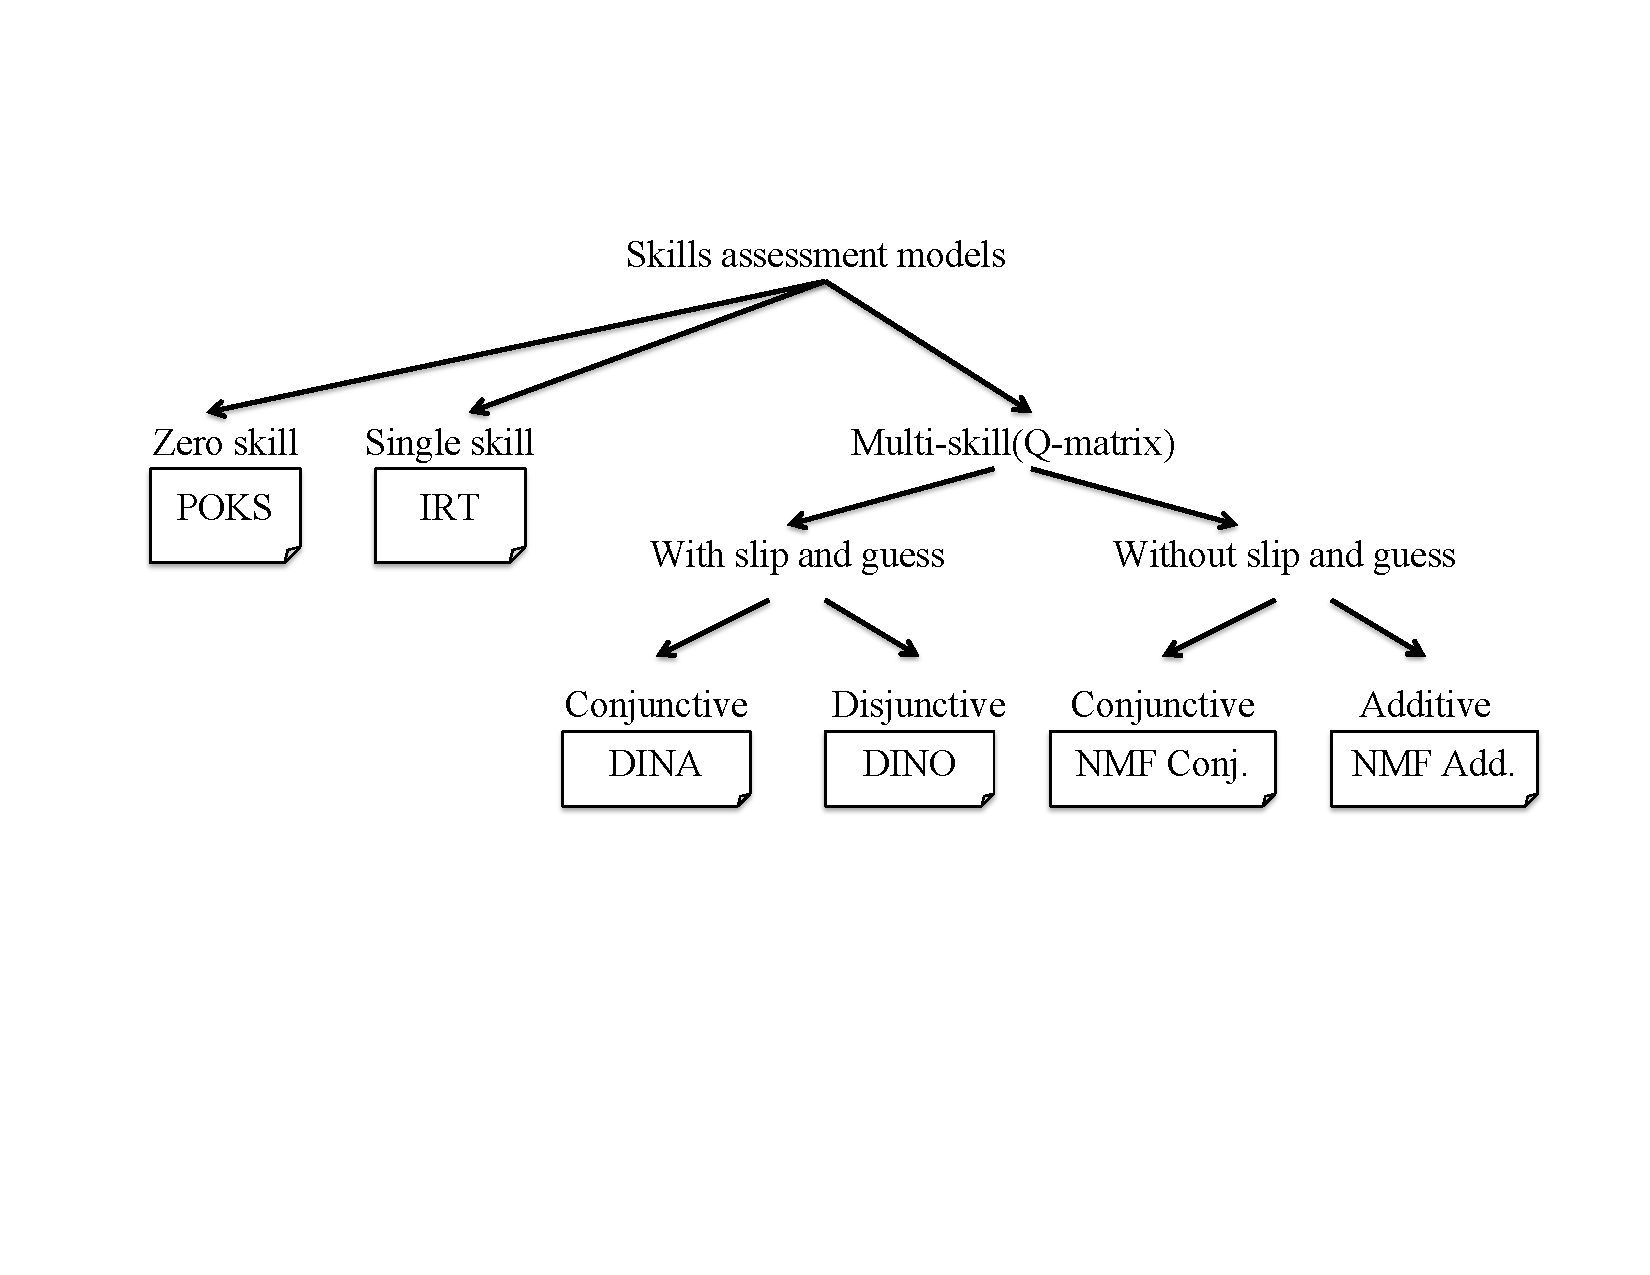
\includegraphics[trim=0.5cm 7cm 0.5cm 3cm,scale =0.4] {images/SkillsAssessments}}
    \end{block}
\begin{overprint}
      \onslide<1>
		\begin{columns}
		\begin{column}{0.35\textwidth}
      		\begin{itemize}
      		\vspace{-0.05cm}
      			\item Number of Skills
	      	\end{itemize}
	      \end{column}
	      \begin{column}{0.7\textwidth}
	      \end{column}
	     \end{columns}
      \onslide<2>
		\begin{columns}
		\begin{column}{0.35\textwidth}
      		\begin{itemize}
      		   	\vspace{-1.1cm}
      			\item Number of Skills
      			\item Q-matrix
	      	\end{itemize}
	      \end{column}
	      \begin{column}{0.7\textwidth}
	      
	      \resizebox{\columnwidth}{1.2cm}{
$\begin{array}{c|c|c}
   \begin{array}{cl}
   &\\
   &\\
   s_{1} : & \text{fraction multiplication}\\
   &\\
   s_{2} : & \text{fraction addition}\\
   &\\
   s_{3} : & \text{fraction reduction}\\
   &\\
   &
\end{array}
&
   \begin{array}{cc}
i_{1} & \frac{4}{\frac{12}{3}}+\frac{3}{5}=\frac{8}{5}\\
 &  \\
i_{2} & \frac{4}{\frac{12}{3}}=\frac{4{\times}3}{12}=\frac{12}{12}=1\\
 &  \\
i_{3} & 1+\frac{3}{5}=\frac{8}{5}\\
 &  \\
i_{4} & 2{\times}\frac{1}{2}=1\\
&
\end{array}
&
\begin{array}{c}
\begin{array}{cc}
 & \textrm{Skills}\\
 & \begin{array}{ccc}
s_{1} & s_{2} & s_{3}\end{array}\\
\mathrm{\begin{sideways}Items\end{sideways}}\begin{array}{c}
i_{1}\\
i_{2}\\
i_{3}\\
i_{4}
\end{array} & \left[\begin{array}{ccc}
1 & 1 & 1\\
1 & 0 & 1\\
0 & 1 & 1\\
1 & 0 & 1
\end{array}\right]
\end{array}\\
\\
\\

\end{array}
\end{array}$
	      }
	      
	      \end{column}
	     \end{columns}
      \onslide<3>
		\begin{columns}
		\begin{column}{0.35\textwidth}
      		\begin{itemize}
      			\item Number of Skills
      			\item Q-matrix 
      			\item Slip and Guess
	      	\end{itemize}
	      \end{column}
	      \begin{column}{0.7\textwidth}
	      \end{column}
	     \end{columns}
	     \onslide<4>
	     		\begin{columns}
		\begin{column}{0.4\textwidth}
      		\begin{itemize}
      		      		   	\vspace{-0.5cm}
      			\item Number of Skills
      			\item \textbf{Q-matrices (types)}%some are based on matrix factorization but others have more adhoc representation
      			\item Slip and Guess
	      	\end{itemize}
	      \end{column}
	      \begin{column}{0.25\textwidth}
	      \begin{enumerate}
	      \item Conjunctive
	      \item Additive 
	      \item Disjunctive
	      \end{enumerate}
	      \end{column}
	      \begin{column}{0.4\textwidth}
	      
	      \resizebox{0.66\columnwidth}{1.2cm}{

$\begin{array}{c}
\begin{array}{cc}
 & \textrm{Skills}\\
 & \begin{array}{ccc}
s_{1} & s_{2} & s_{3}\end{array}\\
\mathrm{\begin{sideways}Items\end{sideways}}\begin{array}{c}
i_{1}\\
i_{2}\\
i_{3}\\
i_{4}
\end{array} & \left[\begin{array}{ccc}
1 & 1 & 1\\
1 & 0 & 1\\
0 & 1 & 1\\
1 & 0 & 1
\end{array}\right]
\end{array}\\
\\
\\

\end{array}$
	      }
	      
	      \end{column}
	     \end{columns}
\end{overprint}
\end{frame}

\newcommand{\tabitem}{~~\llap{\textbullet}~~}
\newcommand\VRule[1][\arrayrulewidth]{\vrule width #1}


\subsection{Presentation terms and concepts}
\begin{frame}\frametitle{Presentation terms and concepts}
\begin{itemize}
\item<1-> \textbf{Performance of a model} over a data set
\item<2-> Model parameters
\item<3-> Performance vector
\item<3-> Performance signature
\item<4-> Performance prototype
\item<5-> Target performance vector
\end{itemize}
\begin{overprint}
\vspace{-2cm}
\onslide<1> \centering 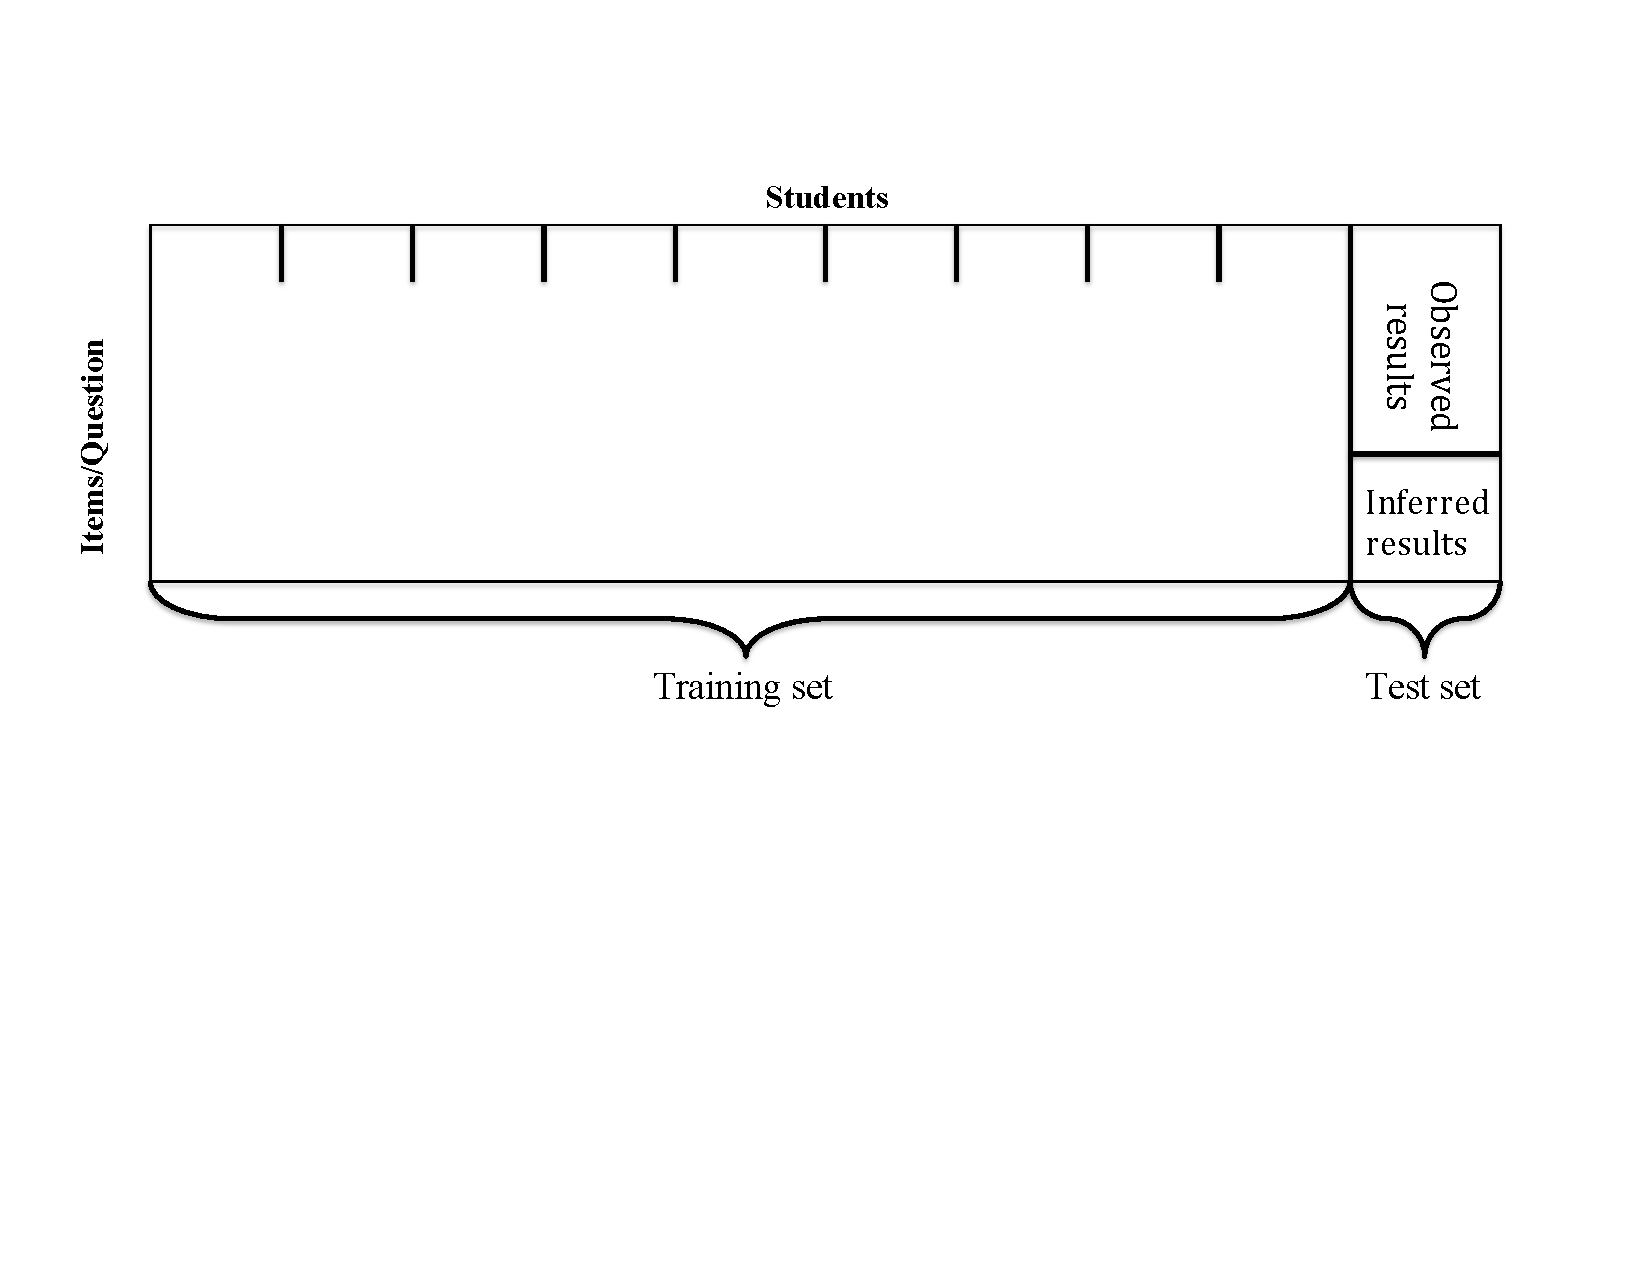
\includegraphics[trim=0cm 8.5cm 2.4cm 2.4cm,clip=true,width=\textwidth]{images/Methodology.pdf}
\onslide<2> \vspace{1cm} \centering 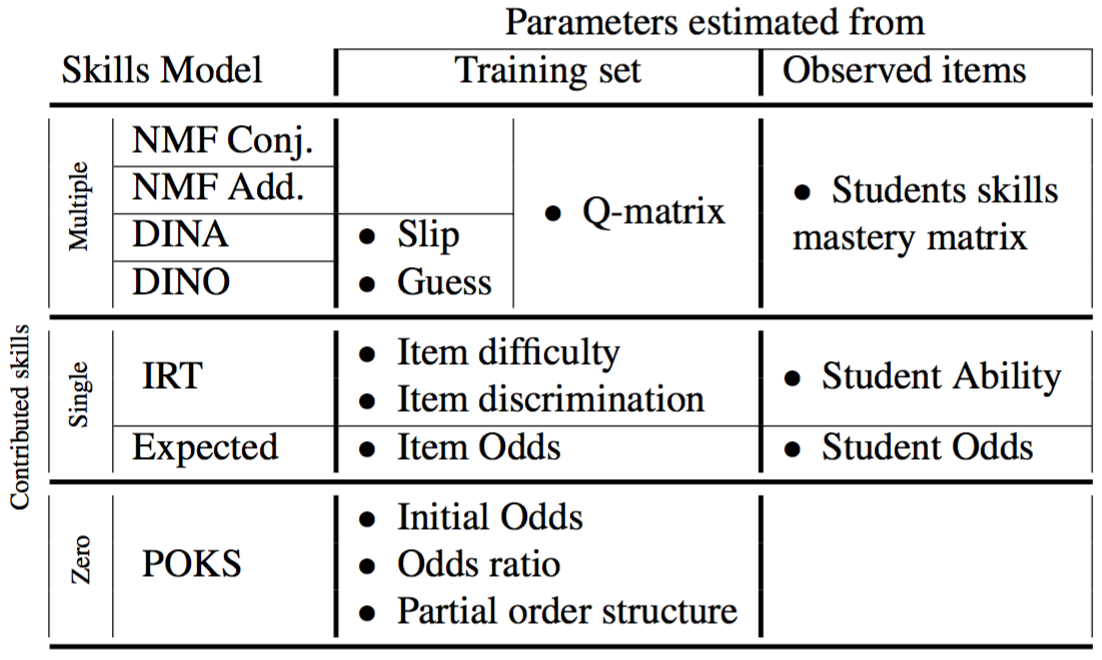
\includegraphics[width=.7\textwidth]{images/Parameters-Model}
\onslide<3>
		\begin{columns}
		\begin{column}{0.5\textwidth}
		 %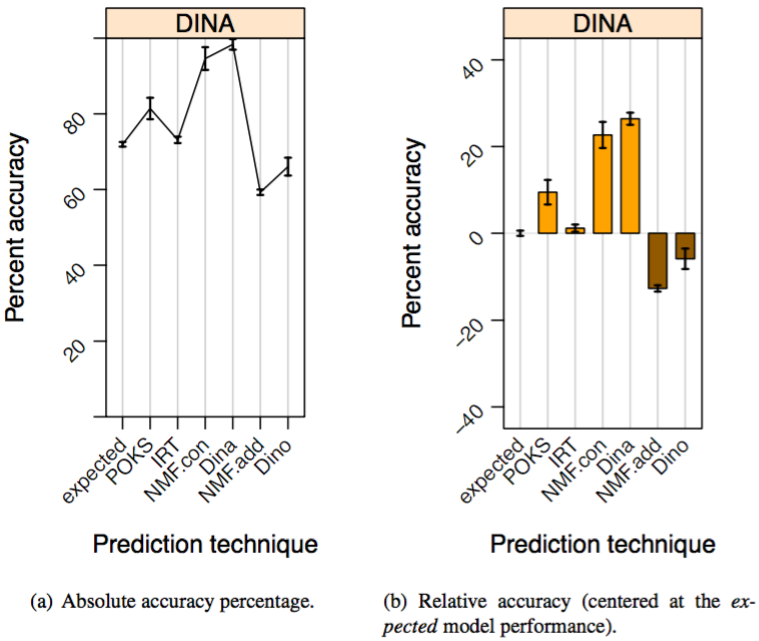
\includegraphics[trim=0cm 0cm 0cm 0cm,clip=true,width=\textwidth]{images/Performance-Presentation}	   
		 \vspace{1.25cm}   
   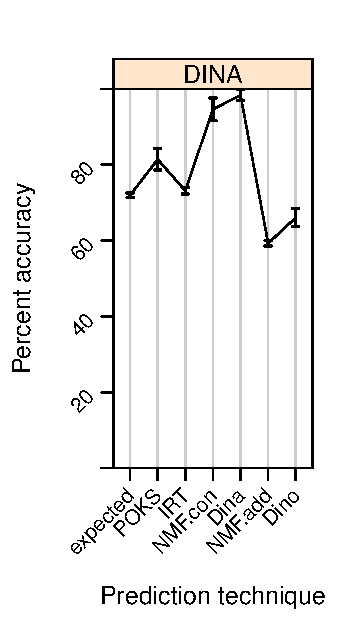
\includegraphics[trim=0cm 0cm 0cm 1.5cm,clip=true,scale =0.55] {images/Predictive-Preformace_Sig.pdf}
   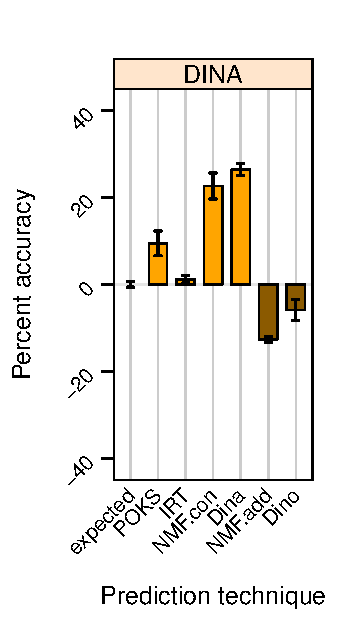
\includegraphics[trim=0cm 0cm 0cm 1.5cm,clip=true,scale =0.55] {images/Predictive-Preformace_Base.pdf}

		 \end{column}
	      \begin{column}{0.5\textwidth}
	      \[\begin{array}{l|c}
	      Model & Performace\\
	      \cline{1-2}
			Expected & 0.72\%\\
			POKS & 0.80\%\\
			IRT & 0.74\%\\
			NMF.Conj & 0.94\%\\
			Dina & 0.99\%\\
			NMF.Add & 0.60\%\\
			Dino & 0.65\%
			\end{array}
			\]
	      \end{column}
	     \end{columns}
\onslide<4>\vspace{3cm} The \textit{performance vector} associated with the synthetic data of a model class.
\onslide<5>\vspace{3cm} The \textit{performance vector} of the real data set to classify.
\end{overprint}
\end{frame}

\section{Main contributions}
\subsection{Experiment 1: Predictive performance}
\begin{frame}\frametitle{Research questions}
\begin{enumerate}
\item \checkmark What is the \textit{performance vector} of student skills assessment models over real and over synthetic data created using the same models?
\begin{itemize}
\item Experiment 1: Predictive \textit{performance vector} of models over real and synthetic data sets
\end{itemize}
\end{enumerate}
\end{frame}


\begin{frame}\frametitle{Datasets}
\centering
\resizebox{7cm}{!}{
\centering
\footnotesize
\begin{tabular}{|l|c|c|r|r|l|}
\hline

%\rowcolor{\color[rgb]{.8,.8,.8}}
\multirow{2}{*}{Data set} & \multicolumn{3}{c|}{Number of} & {\parbox{6ex}{\center Mean\\Score}} & \multirow{2}{*}{Q-matrix}\tabularnewline
\cline{2-4} 
%\rowcolor{\color[rgb]{.8,.8,.8}}
 & Skills & Items & Students &  & \tabularnewline
\hline
\hline
%\rowcolor{\color[rgb]{.9,.9,.9}}
\multicolumn{6}{|c|}{\textit{Synthetic}}\\
\hline
\hline
1.Random & 7 & 30 & 700 &0.75& $\mathbf{Q}_{01}$\tabularnewline
\hline
2.POKS & 7 & 20 & 500 &0.50 & $\mathbf{Q}_{02}$\tabularnewline
\hline
3.IRT-2PL & 5 & 20 & 600 &0.50& $\mathbf{Q}_{03}$\tabularnewline
\hline
4.DINA & 7 & 28 & 500 &0.31& $\mathbf{Q}_5$\tabularnewline
\hline
5.DINO & 7 & 28 & 500 &0.69& $\mathbf{Q}_6$\tabularnewline
\hline
\multicolumn{6}{|l|}{Linear (Matrix factorization)}\\
\hline
6.~~~Conj. & 8 & 20 & 500 &0.24& $\mathbf{Q}_1$\tabularnewline
\hline
7.~~~Comp. & 8 & 20 & 500 &0.57& $\mathbf{Q}_1$ \tabularnewline
\hline
\hline
%\rowcolor{\color[rgb]{.9,.9,.9}}
\multicolumn{6}{|c|}{\textit{Real}}\\
\hline
\hline
8.Fraction & 8 & 20 & 536 &0.53& $\mathbf{Q}_1$\tabularnewline
\hline
9.Vomlel & 6 & 20 & 149 &0.61& $\mathbf{Q}_4$\tabularnewline
\hline
10.ECPE & 3 & 28 & 2922 &0.71& $\mathbf{Q}_3$\tabularnewline
\hline
\multicolumn{6}{|l|}{Fraction subsets and variants of $\mathbf{Q}_{1}$}\\
\hline
11.~~~1 & 5 & 15 & 536 &0.53& $\mathbf{Q}_{10}$\tabularnewline
\hline
12.~~~2/1 & 3 & 11 & 536 &0.51& $\mathbf{Q}_{11}$\tabularnewline
\hline
13.~~~2/2 & 5 & 11 & 536 &0.51& $\mathbf{Q}_{12}$\tabularnewline
\hline
14.~~~2/3 & 3 & 11 & 536 &0.51& $\mathbf{Q}_{13}$\tabularnewline
\hline
\end{tabular}}
\end{frame}

\begin{frame}\frametitle{Predictive performance of models over synthetic datasets}
\vspace{-0.5cm}
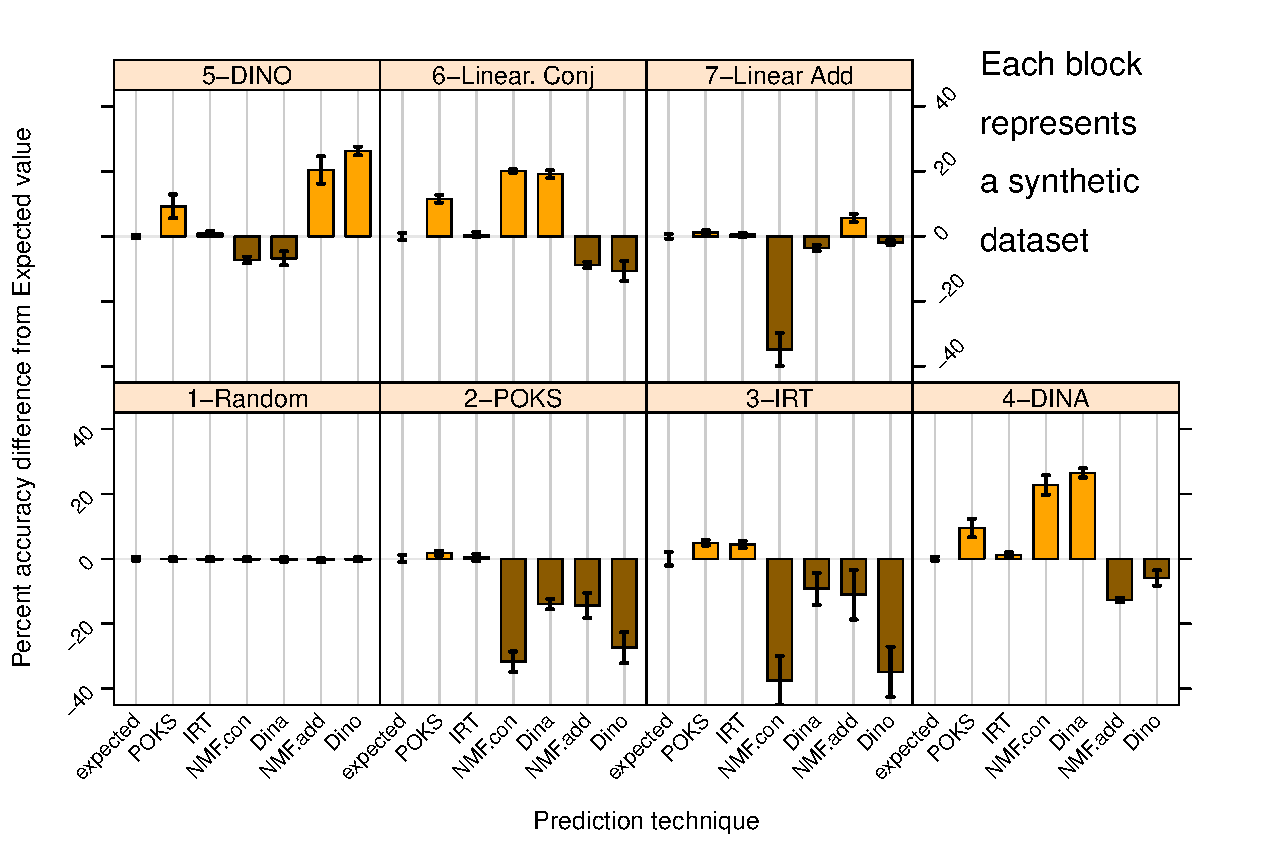
\includegraphics[scale =0.45] {images/Syn}
\begin{overprint}
     \onslide<1> The random data set has a flat performance across techniques 
     %%%which corresponds to the dominant class prediction. 
      \onslide<2> \small The highest performance is for the generative model behind the dataset
%The highest performance is for the skills assessment technique that is the same as the generative model behind the dataset%%%%the generative model behind the data set is the same as the skills assessment technique, the corresponding technique’s performance is the best, or close to the best.
	  \onslide<3> \small Data sets have unique pattern of performance vector across models
	  \onslide<4> The capacity of recognizing a data set’s true model relies on this uniqueness characteristic
\end{overprint}
\end{frame}

\begin{frame}\frametitle{Predictive performance of models over real datasets}
\vspace{-0.5cm}
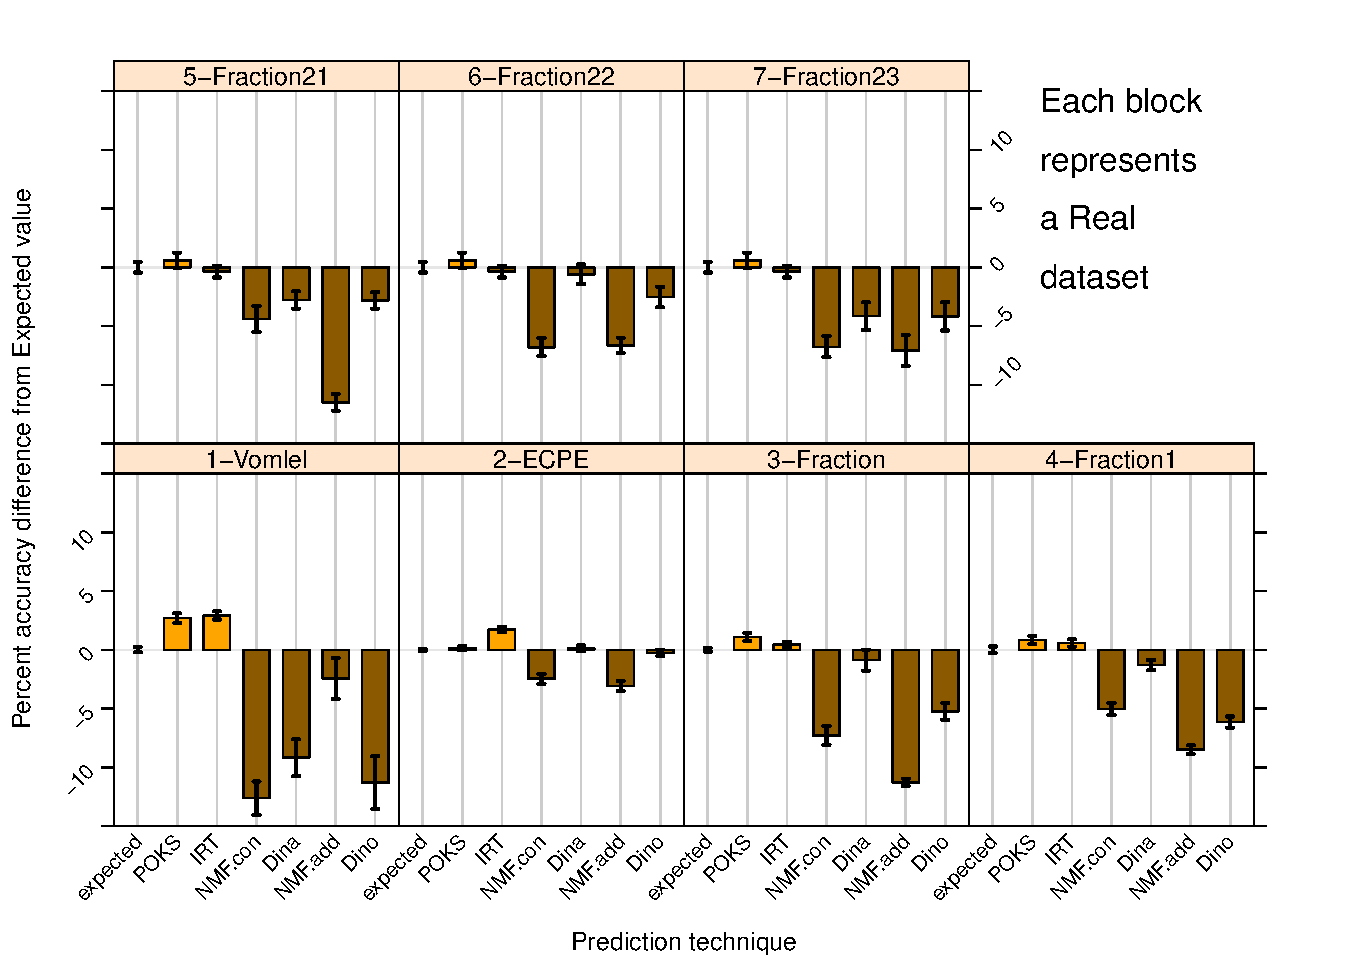
\includegraphics[scale =0.4] {images/Real}
\begin{overprint}
      \onslide<1> In most cases, the best performer is close to the baseline %many methods are not doing better than expected value
      \onslide<2> The pattern of the Fraction performance data set repeats over its subsets %Fraction-1, Fraction-2/1 and Fraction-2/2, in spite of the different number of skills and different subsets of questions
      %this similarity among Fraction data set and its derivative suggests that in spite of the model differences (different Q-matrices and item subsets), the performance signature remains constant across these data sets.
      \onslide<3> None of the real data sets show the large variance and the differences found in the synthetic data sets models %Scles are 4 times bigger
\end{overprint}
\end{frame}

\begin{frame}\frametitle{Vector space of accuracy performances}
\begin{itemize}
\item Performance vectors of datasets in columns(Data points in the performance space)
\end{itemize}
\resizebox{\columnwidth}{!}{
\begin{tabular}{lccccccc}
  \toprule
  \multicolumn{1}{c}{\multirow{2}{*}{\textbf{Model}}} & \multicolumn{7}{c}{\textbf{Synthetic data set }} \\
  \cline{2-8}
  & \multicolumn{1}{c}{{\textit{Random}}} & \multicolumn{1}{c}{{POKS}} & \multicolumn{1}{c}{{IRT}} & \multicolumn{1}{c}{{DINA}} & \multicolumn{1}{c}{{DINO}} & \multicolumn{1}{c}{{Linear .Conj}} & \multicolumn{1}{c}{{Linear .Comp}} \\ 
  \hline
  \textit{Expected} & \textbf{0.75} & 0.91 & 0.90 & 0.72 & 0.72 & 0.78 & 0.93 \\ 
  POKS & 0.75 & \textbf{0.94} & 0.94 & 0.81 & 0.81 & 0.90 & 0.94 \\ 
  IRT & 0.75 & 0.91 & \textbf{0.95} & 0.73 & 0.73 & 0.79 & 0.89 \\ 
  DINA & 0.75 & 0.77 & 0.81 & \textbf{1.00} & 0.65 & \textbf{0.98} & 0.89 \\ 
  DINO & 0.75 & 0.63 & 0.56 & 0.66 & \textbf{1.00} & 0.68 & 0.91 \\ 
  NMF.Conj & 0.75& 0.59 & 0.53 & 0.95 & 0.65 & 0.97 & 0.58 \\ 
  NMF.Comp & 0.75 & 0.76 & 0.79 & 0.59 & 0.93 & 0.70 & \textbf{0.98} \\ 
  \bottomrule
\end{tabular}}
\vspace{.7cm}

The diagonal generally displays the best performance %the diagonal (in bold face, except for one, corresponding to the match between the underlying synthetic model and the model performance) generally displays the best perfor- mance since it corresponds to the alignment of the model and the ground truth behind the data.

\end{frame}

\subsection{Experiment 2: Sensitivity of the Model performance}
\begin{frame}\frametitle{Research questions}
\begin{enumerate}
\item \checkmark What is the \textit{performance vector} of student skills assessment models over real and over synthetic data created using the same models?
\begin{itemize}
\item Experiment 1: Predictive performance of models over real and synthetic data sets
\end{itemize}
\item \textbf{Is the \textit{performance vector} unique to each synthetic data type (data from the same ground truth model)?}
\begin{itemize}
\item Experiment 2: Sensitivity of the Model performance over different data generation parameters
\end{itemize}
Are they stable in addition to be unique?
\end{enumerate}
\end{frame}

\begin{frame}\frametitle{Variation of sample size over synthetic data sets}
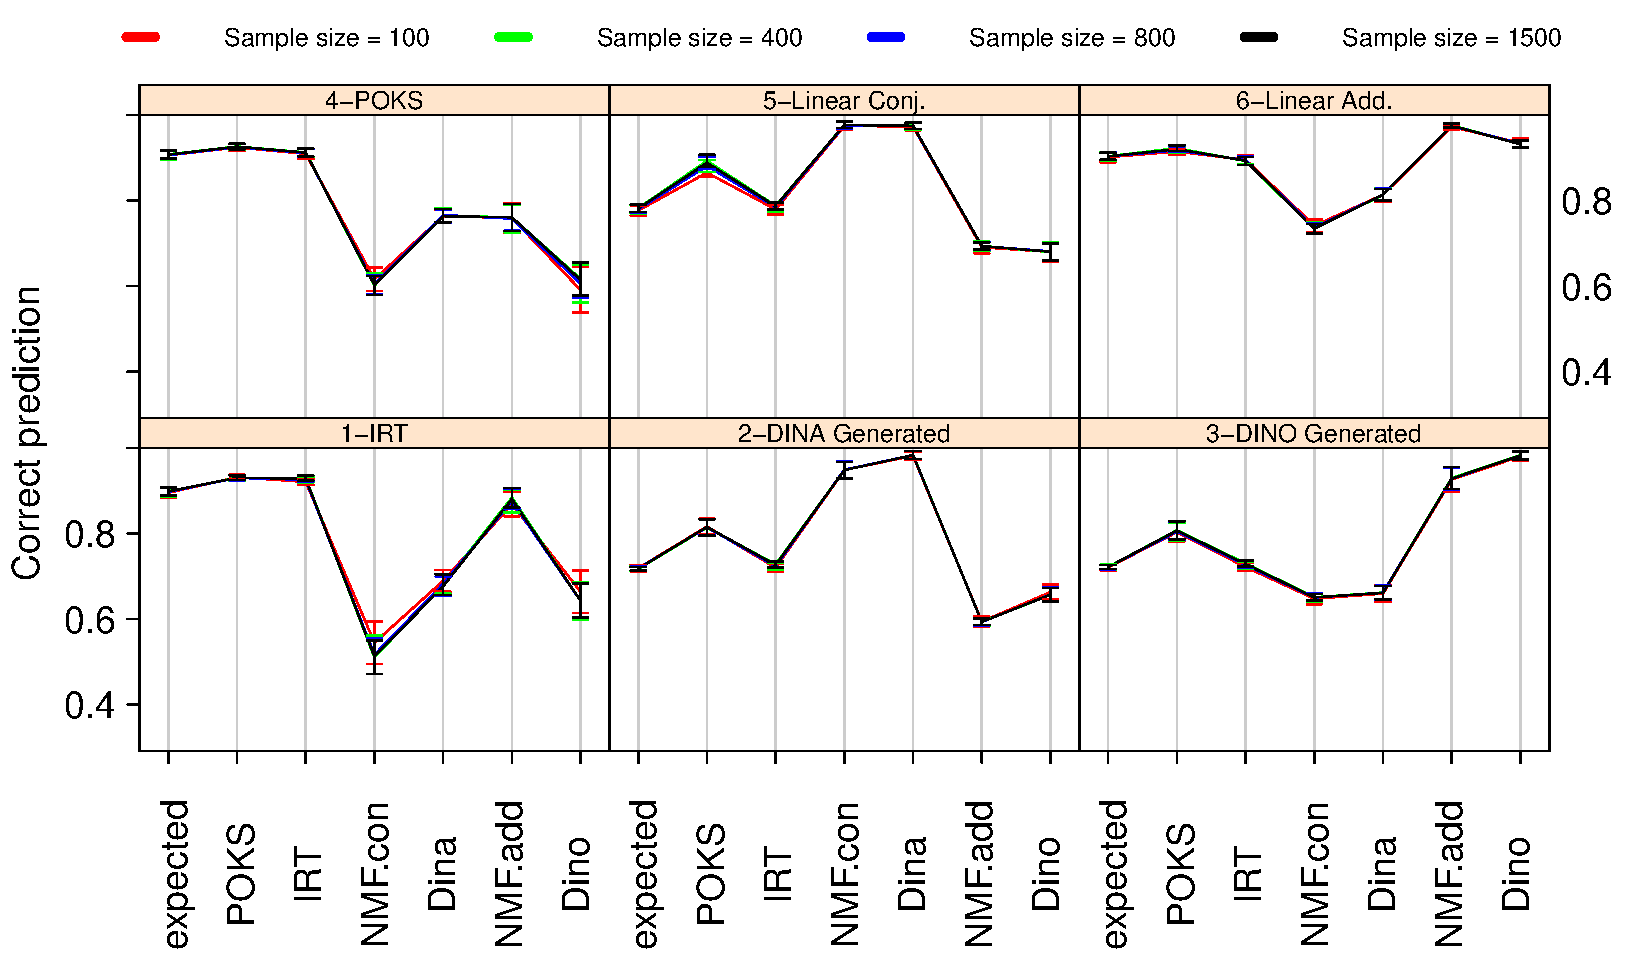
\includegraphics[scale =0.37] {images/SampleSize}
\begin{overprint}
      \onslide<1> Obviously, the signature pattern did not change significantly for some parameters such as \textbf{Sample size}.
\end{overprint}
\end{frame}

\begin{frame}\frametitle{Variation of number of items over synthetic data sets}
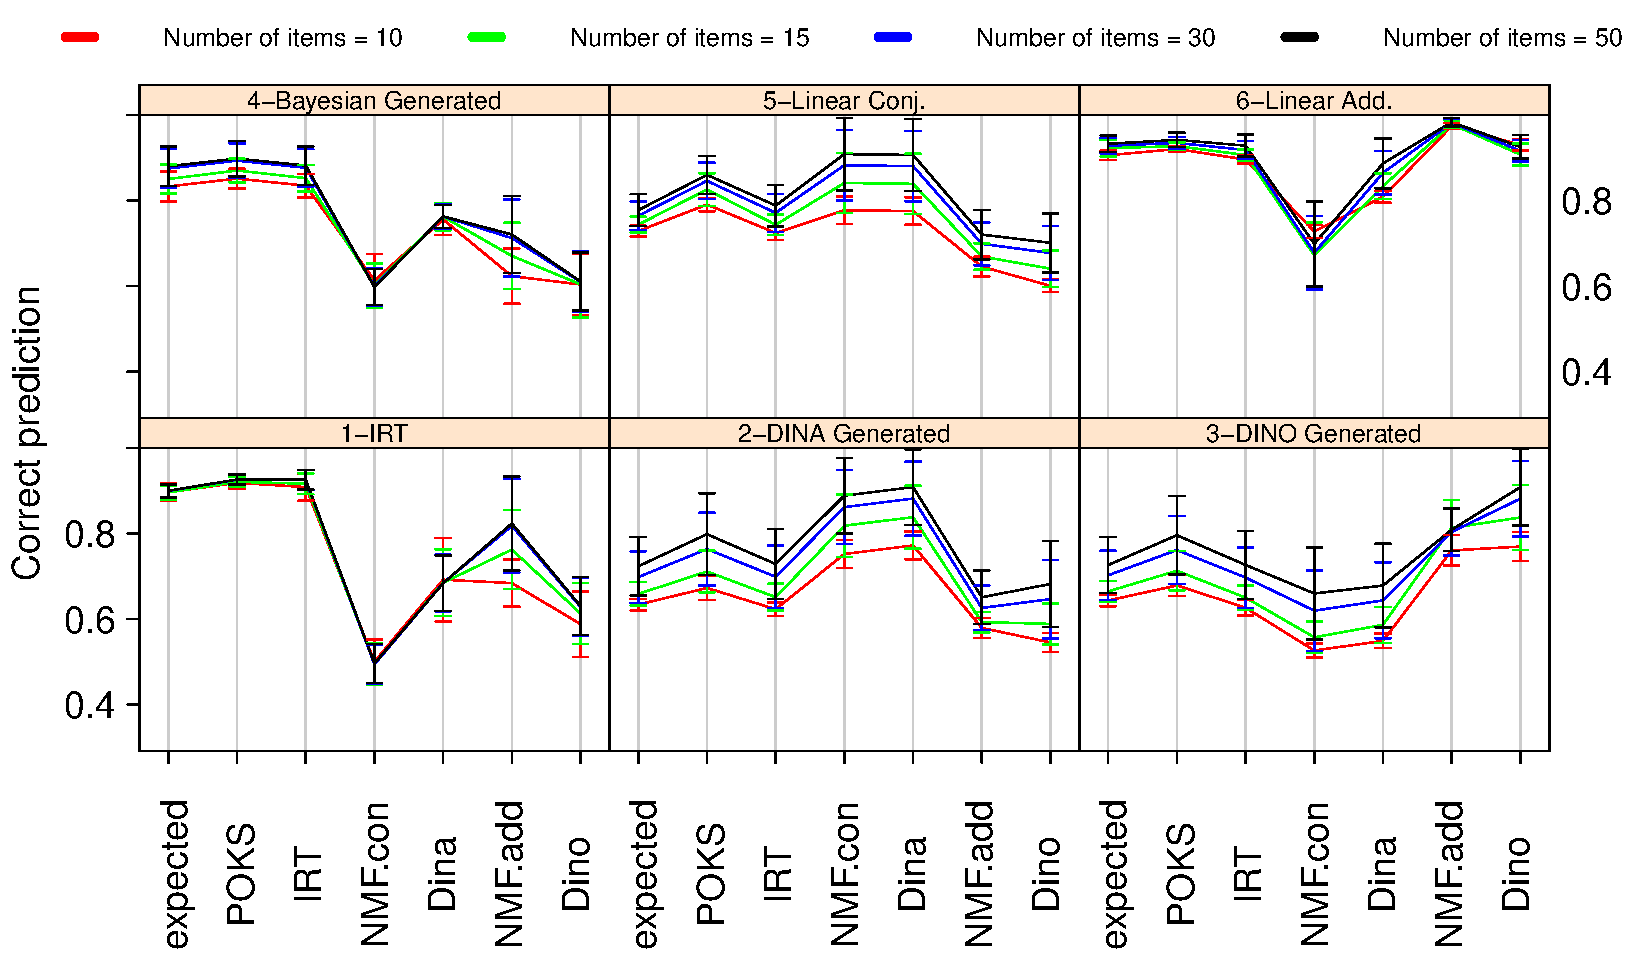
\includegraphics[scale =0.37] {images/numberofitems}
\begin{overprint}
	  \onslide<1> Even for synthetic data the performance of the ground truth model should not necessarily be close to 100\%.
      \onslide<2> The Performance signature shifts down once the number of items degrades.
\end{overprint}
\end{frame}

\begin{frame}\frametitle{Data specific parameters}
\begin{enumerate}
\item Sample size (Number of students)
\item Number of items
\item Number of latent skills
\item Item score variance 
\item Student score variance
\item Average success rate\pause
\end{enumerate}
Conclusion :
\begin{itemize}
      \item Data specific parameters can potentially influence the performance of a model%the best performer may not be the model that is most representative of the ground truth, but instead it may be the result of contextual factors that make this model outperform the ground truth one.
	  \item For better comparison of the results, we can also consider \textbf{data specific parameters} of the real data in the generation process%we can also consider data specific parameters of the real data in the generation process to make a better comparison of the results.
\end{itemize}
\end{frame}

\subsection{Experiment 3: Signature Approach}
\begin{frame}\frametitle{Research questions}
\begin{enumerate}
\item \checkmark What is the \textit{performance vector} of student skills assessment models over real and over synthetic data created using the same models?
\begin{itemize}
\item Experiment 1: Predictive performance of models over real and synthetic data sets
\end{itemize}
\item \checkmark Is the \textit{performance vector} unique to each synthetic data type (data from the same ground truth model)?
\begin{itemize}
\item Experiment 2: Sensitivity of the Model performance over different data generation parameters
\end{itemize}
\item \textbf{Can the \textit{performance vector} be used to define a method to reliably identify the ground truth behind the synthetic data?}
\begin{itemize}
\item Experiment 3: Model selection based on performance vector classification
\end{itemize}
\end{enumerate}
\end{frame}

\begin{frame}\frametitle{Signature framework}
This approach relies on generating synthetic datasets
\begin{overprint}
\onslide<1> 
		\begin{columns}
		\begin{column}{0.7\textwidth}
		\vspace{-0.8cm}
			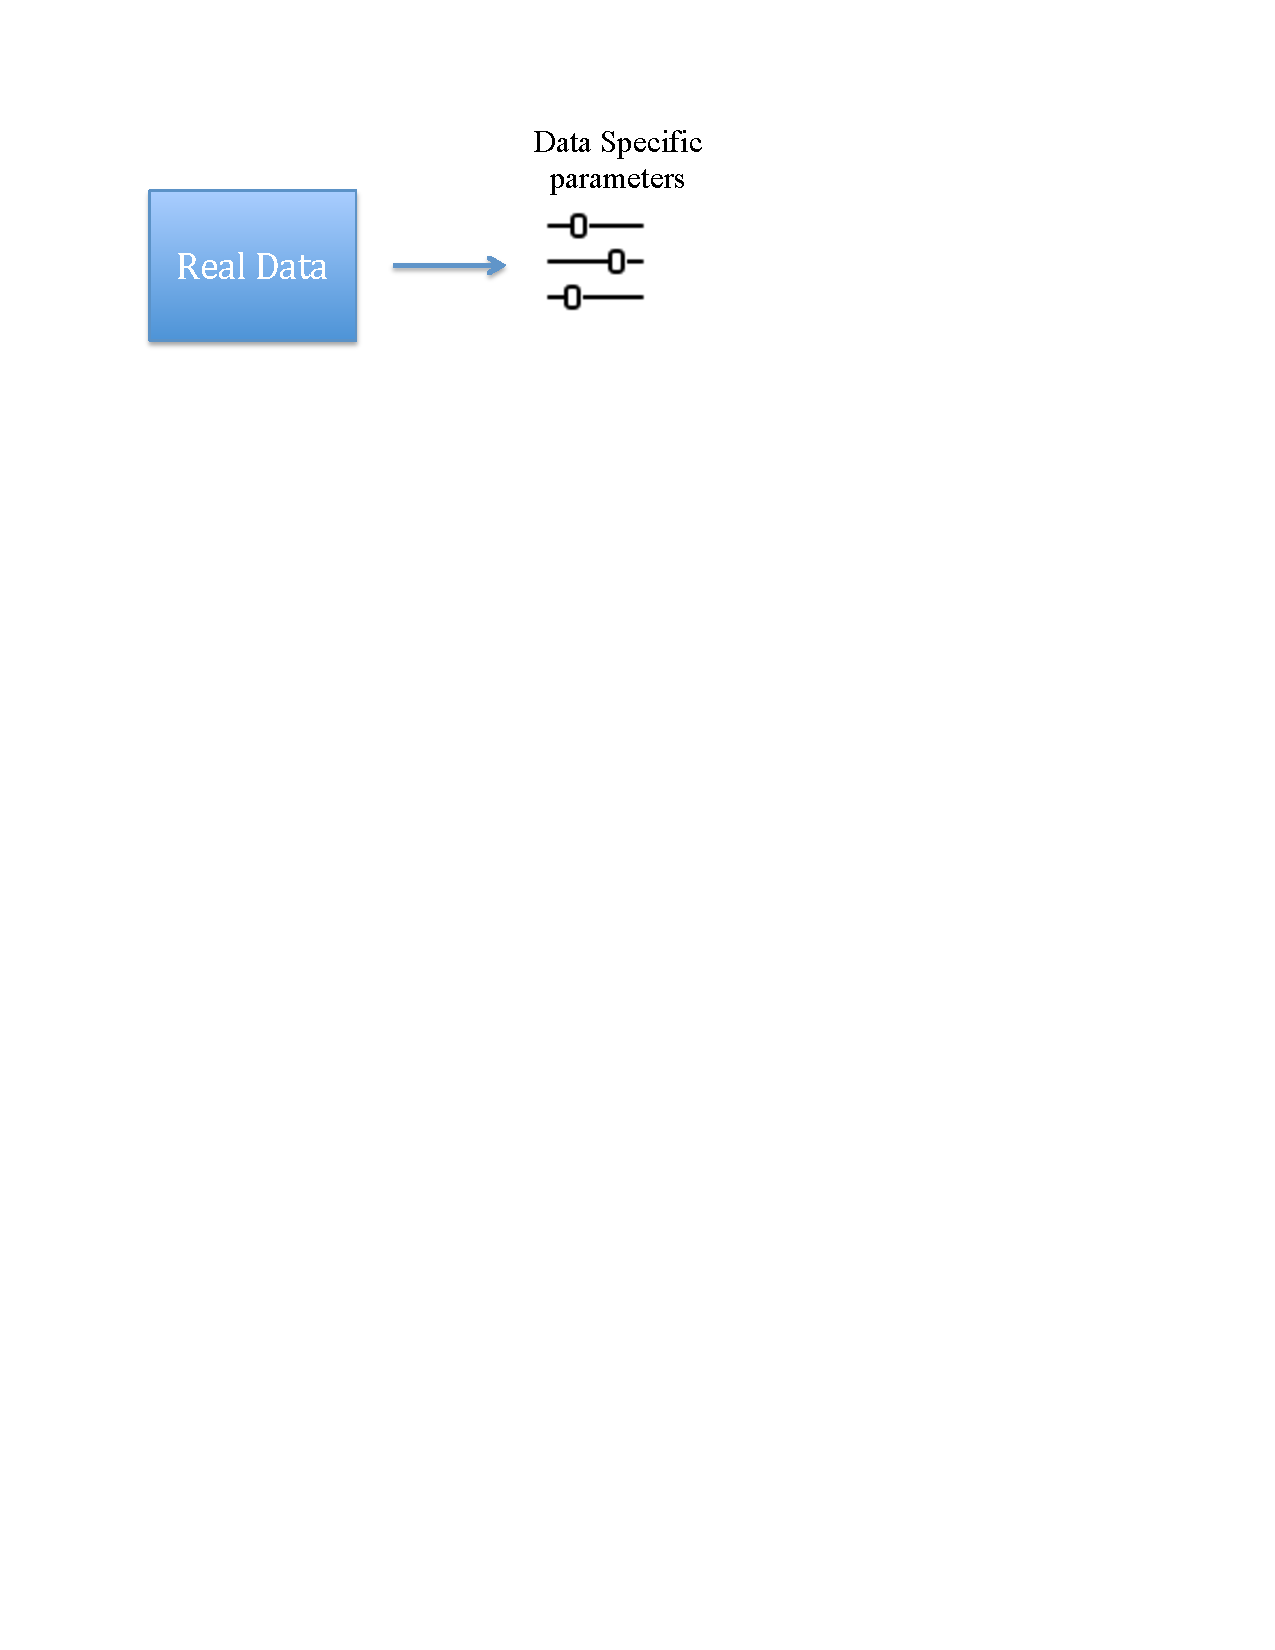
\includegraphics[trim=1cm 10cm 1cm 1cm,scale=0.43]{images/Approach1.pdf}
		\end{column}
		\begin{column}{0.3\textwidth}
		\end{column}
		\end{columns}
\onslide<2> 		\begin{columns}
		\begin{column}{0.7\textwidth}
		\vspace{-0.8cm}
			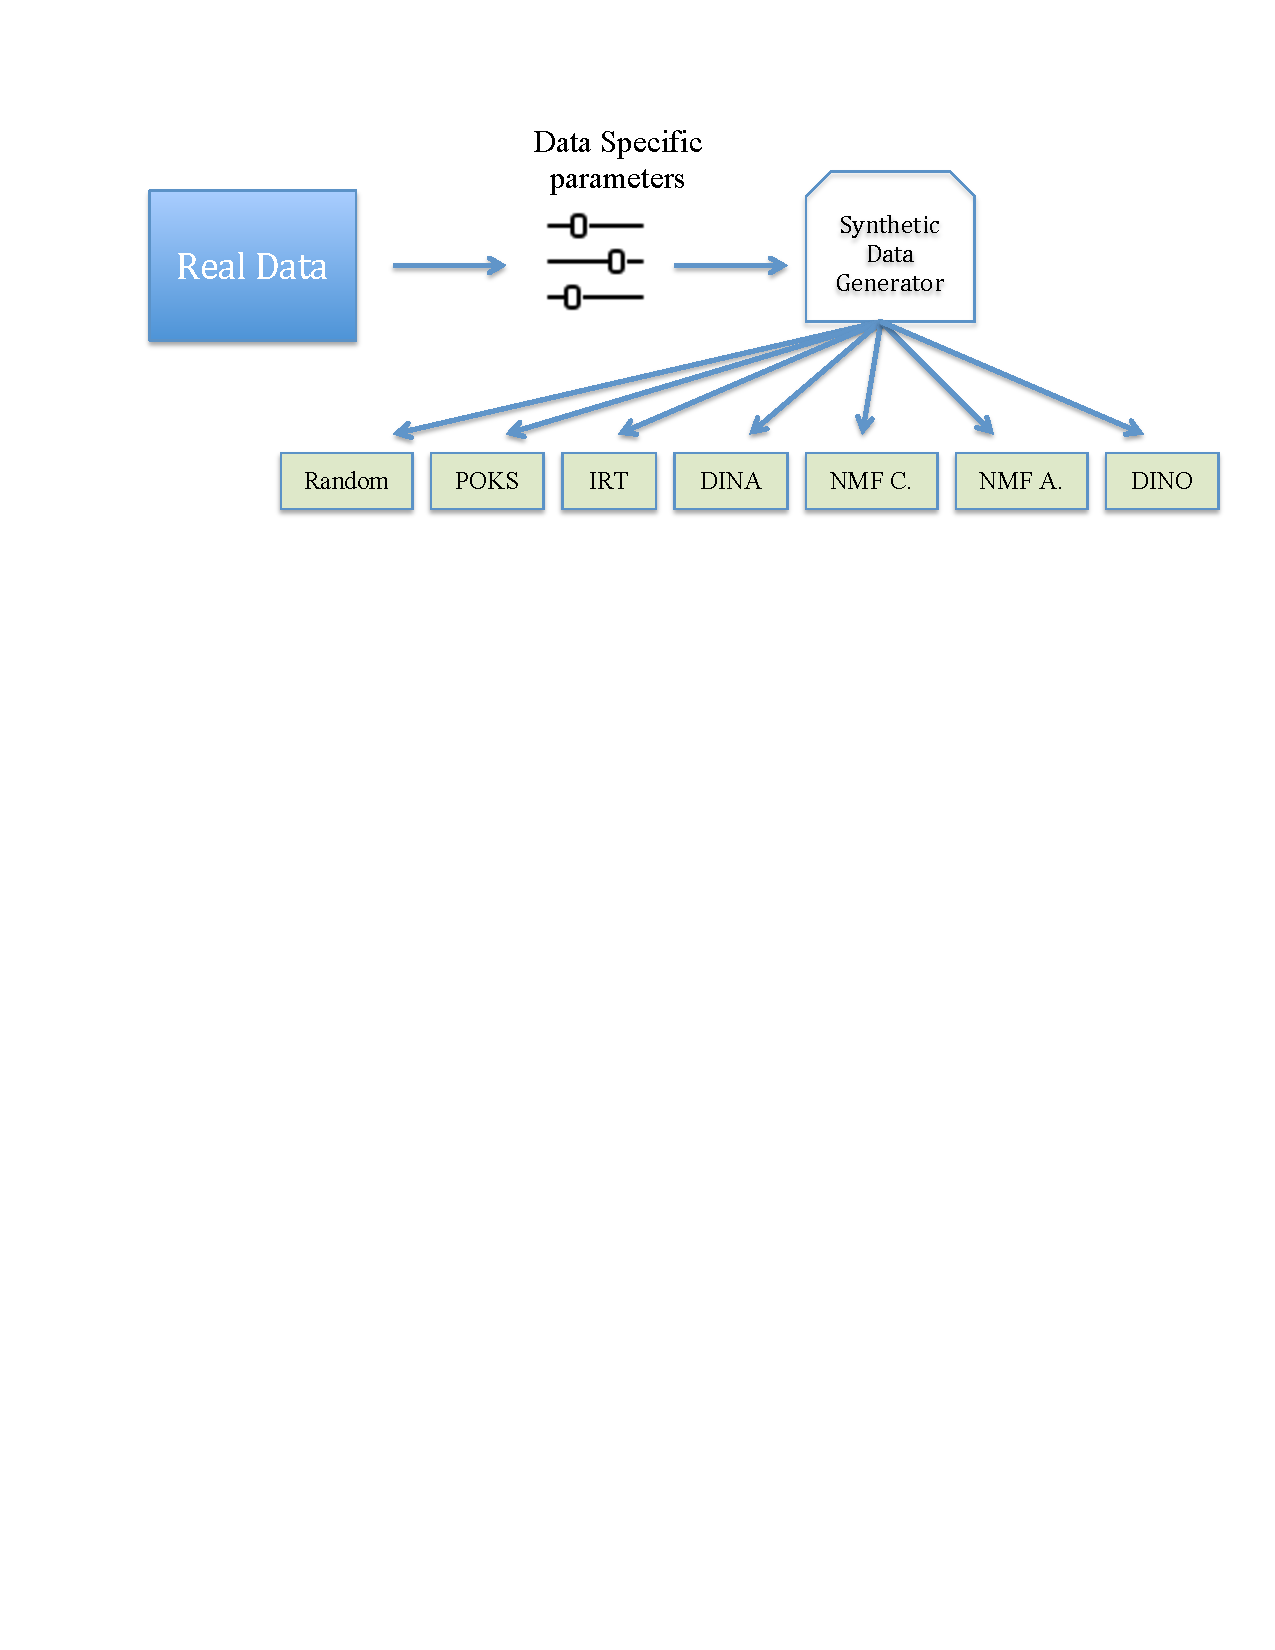
\includegraphics[trim=1cm 10cm 1cm 1cm,scale=0.43]{images/Approach2.pdf}
		\end{column}
		\begin{column}{0.3\textwidth}
		\end{column}
		\end{columns}
		\onslide<3> 		\begin{columns}
		\begin{column}{0.7\textwidth}
			\vspace{-0.8cm}
			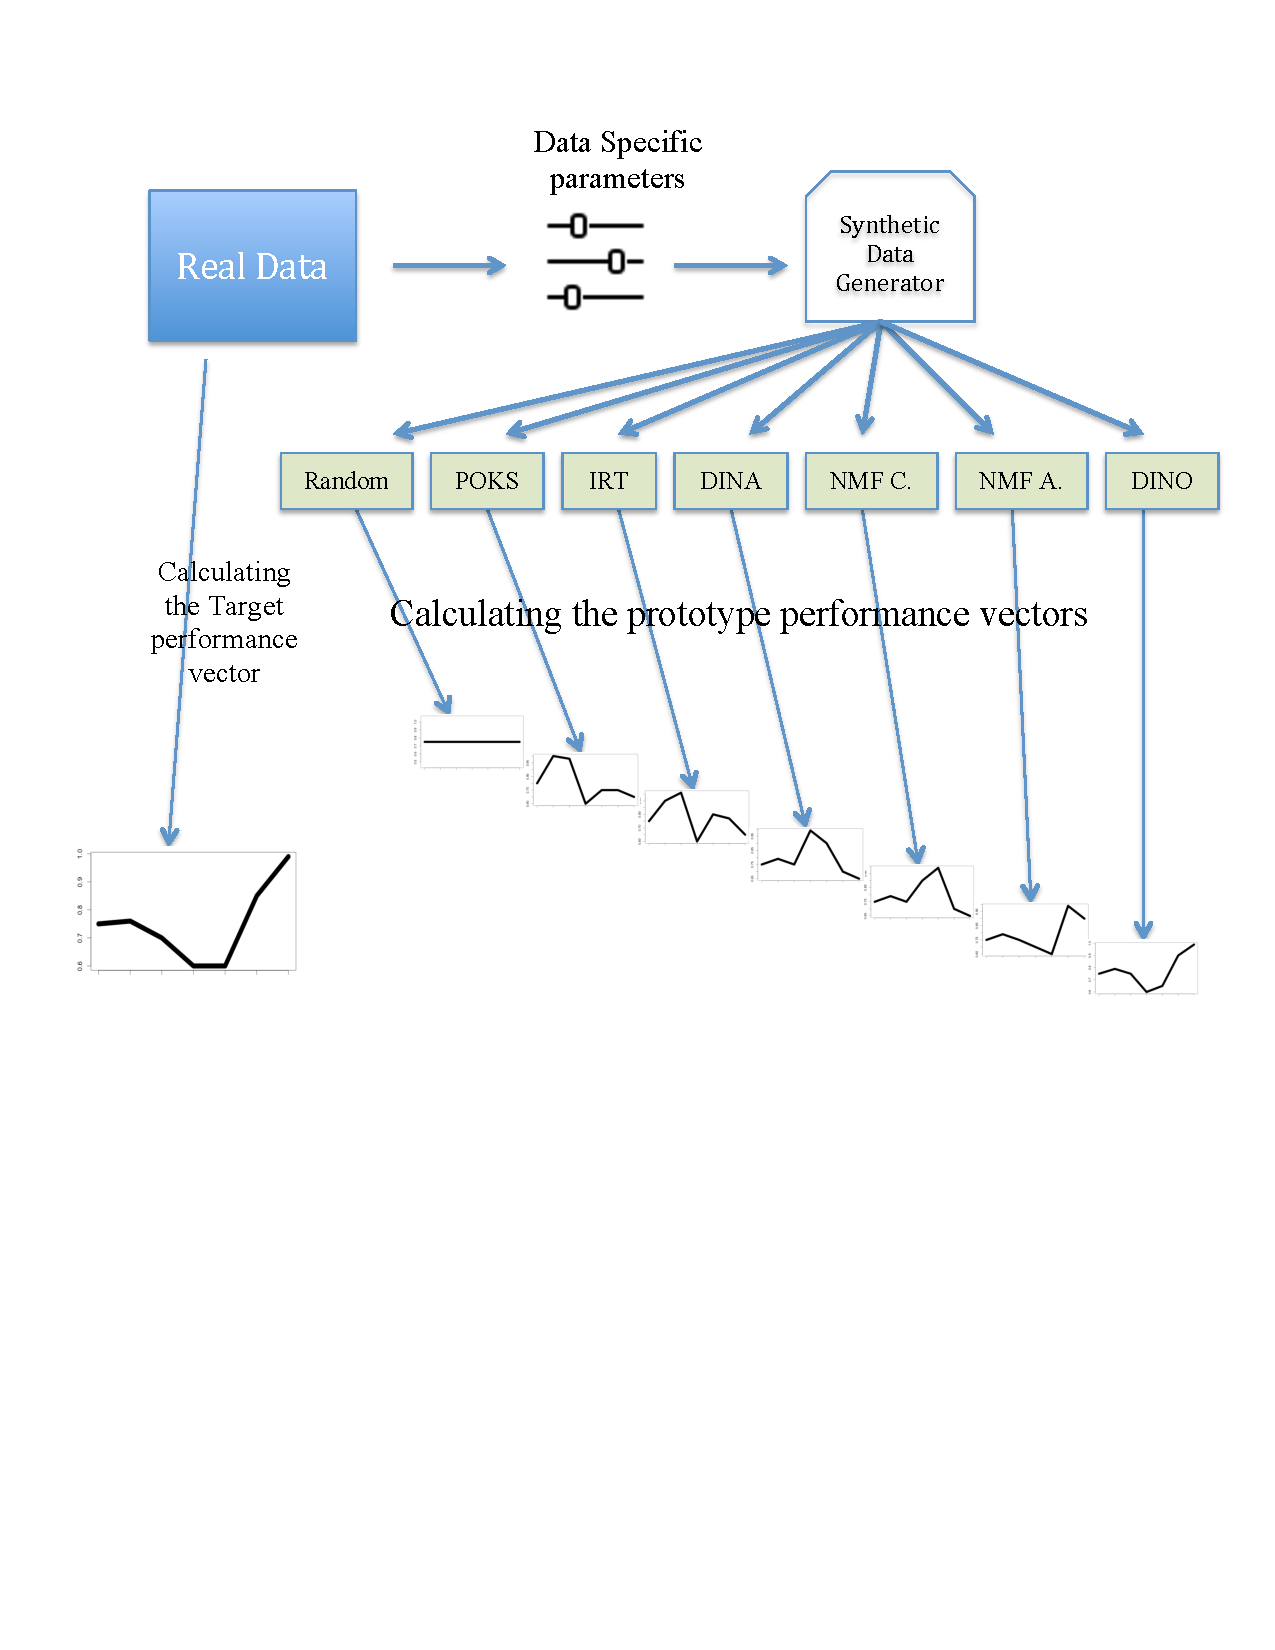
\includegraphics[trim=1cm 10cm 1cm 1cm,scale=0.43]{images/Approach3.pdf}
		\end{column}
		\begin{column}{0.3\textwidth}
			\hspace{1.5cm}Recall
          
          \vspace{1cm}
           \rightline{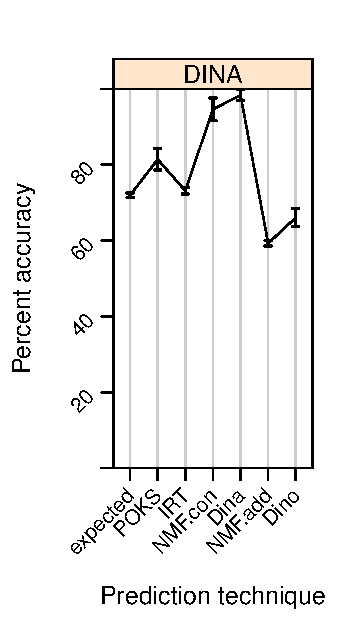
\includegraphics[trim=0cm 0cm 0cm 1.5cm,clip=true,scale =0.5] {images/Predictive-Preformace_Sig.pdf}}


		\end{column}
		\end{columns}
		\onslide<4> 		\begin{columns}
		\begin{column}{0.7\textwidth}
			\vspace{-0.8cm}			
			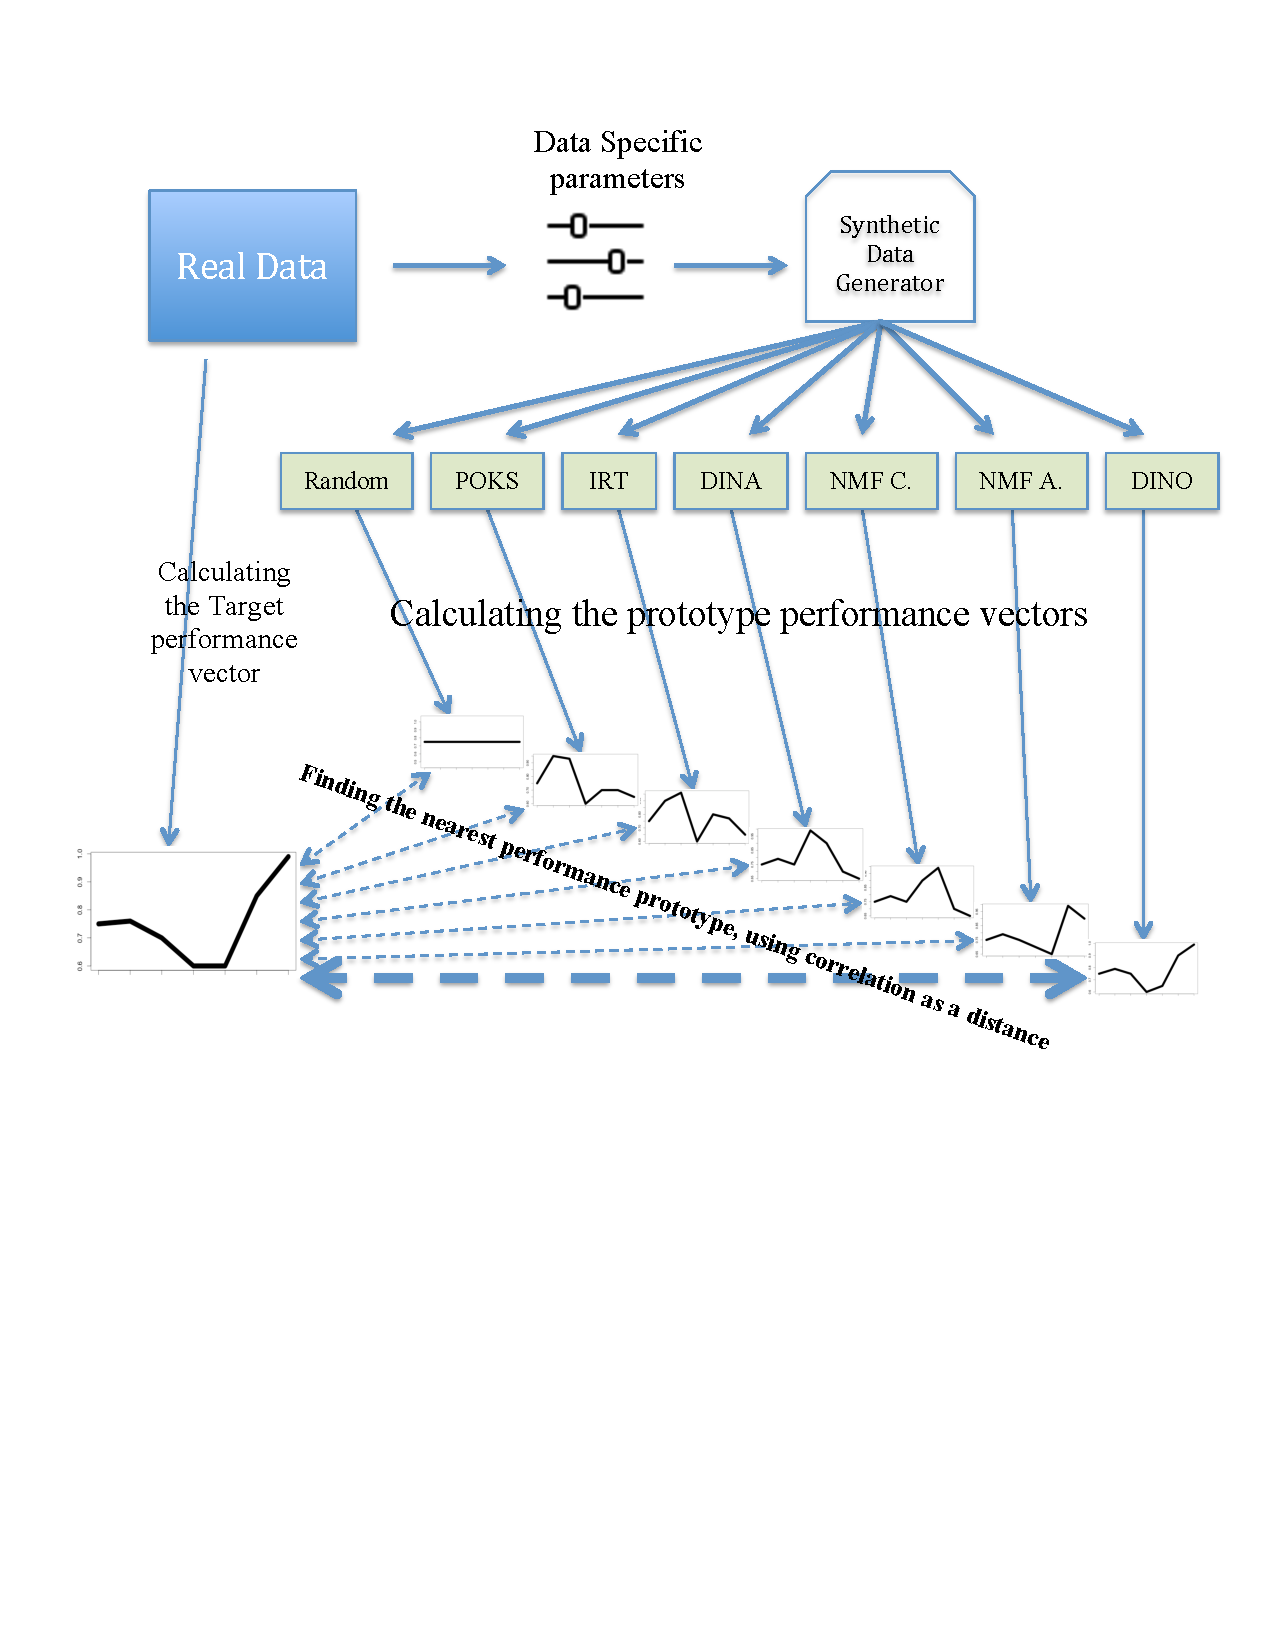
\includegraphics[trim=1cm 10cm 1cm 1cm,scale=0.43]{images/Approach4.pdf}
		\end{column}
		\begin{column}{0.3\textwidth}
		\end{column}
		\end{columns}\end{overprint}
\end{frame}

\begin{frame}\frametitle{Pool of synthetic datasets}
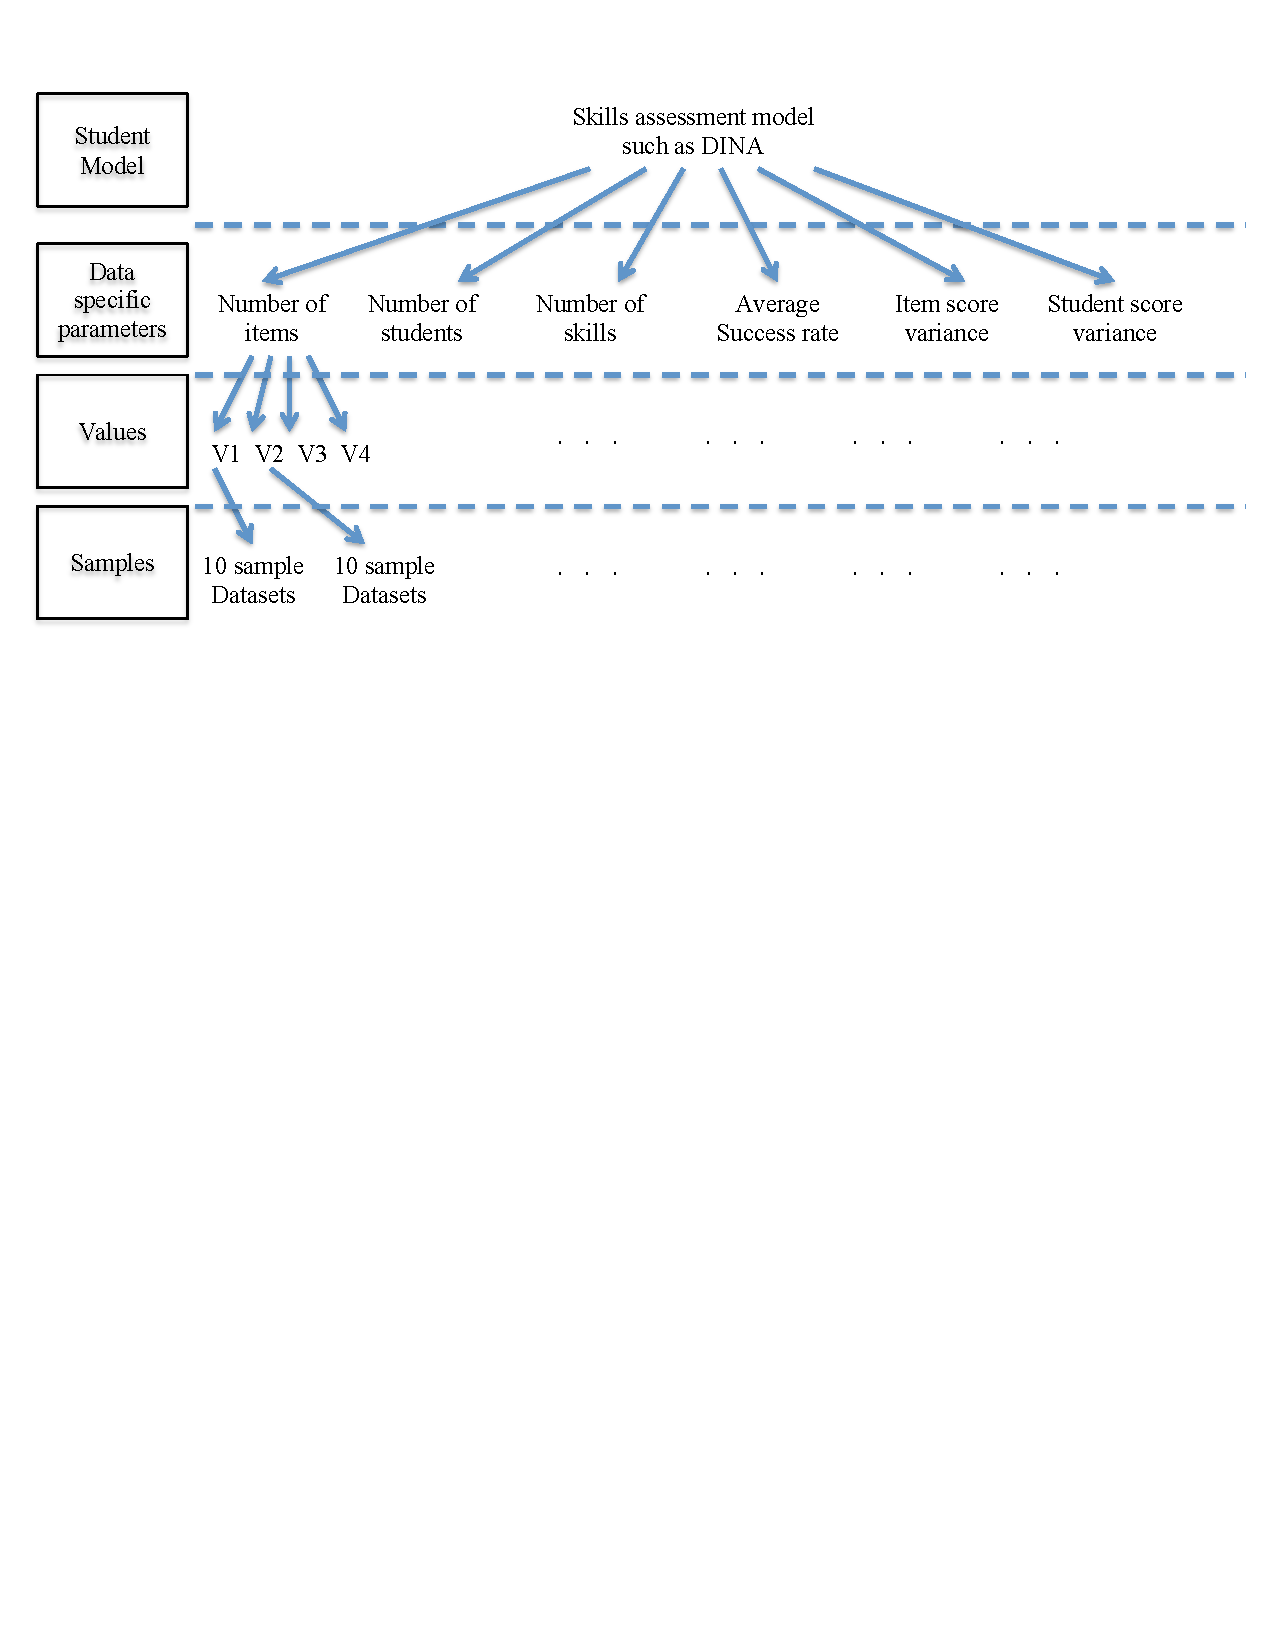
\includegraphics[trim=1cm 17cm 1cm 1cm,scale=0.55]{images/Data-Gen-Break-Down.pdf}
\begin{overprint}
\onslide<1> There exists 6 skills assessment models 
\onslide<2> There exists 6 skills assessment models X 6 data specific parameters 
\onslide<3> There exists 6 skills assessment models X 6 data specific parameters~X 4 values 
\onslide<4> There exists 6 skills assessment models X 6 data specific parameters~X 4 values X 10 samples = 1440 samples in the pool
\end{overprint}
\end{frame}

\begin{frame}\frametitle{Degree of similarity between six synthetic datasets based on the correlation}
\resizebox{\columnwidth}{!}{\begin{tabular}{c|c|c|c|c|c|c|c|}
\multicolumn{2}{c}{} & \multicolumn{6}{c}{Synthetic Datasets} \tabularnewline
\multicolumn{8}{c}{} \tabularnewline
\cline{3-8} 
\multicolumn{2}{c|}{} & POKS & IRT & NMF Conj. & DINA & NMF Add. & DINO\tabularnewline
\cline{2-8}
\cline{2-3}
&POKS & \textbf {0.96} & \multicolumn{1}{|c}{} & \multicolumn{1}{c}{} & \multicolumn{1}{c}{} & \multicolumn{1}{c}{}\tabularnewline
\cline{2-4}
&IRT & 0.86 & \textbf {0.96} & \multicolumn{1}{|c}{} & \multicolumn{1}{c}{} & \multicolumn{1}{c}{} & \multicolumn{1}{c}{}\tabularnewline
\cline{2-5}
&NMF Conj. & 0.22 & -0.20 & \textbf {0.96} & \multicolumn{1}{|c}{} & \multicolumn{1}{c}{} & \multicolumn{1}{c}{}\tabularnewline
\cline{2-6}
&DINA & 0.02 & -0.40 & 0.94 & \textbf {0.96} & \multicolumn{1}{|c}{} & \multicolumn{1}{c}{}\tabularnewline
\cline{2-7}
&NMF Add. & 0.44 & 0.75 & -0.62 & -0.73 & \textbf {0.93} & \multicolumn{1}{|c}{}\tabularnewline
\cline{2-8}
\multicolumn{1}{c|}{\multirow{-6}{*}{\begin{sideways}Synthetic Datasets\end{sideways}}}&DINO & -0.15 & 0.20 & -0.70 & -0.69 & 0.63 & \textbf {0.95}\tabularnewline
\cline{2-8}
\multicolumn{1}{c}{} &\multicolumn{1}{c}{} & \multicolumn{1}{c}{} & \multicolumn{1}{c}{} &\multicolumn{1}{c}{} & \multicolumn{1}{c}{} & \multicolumn{1}{c}{} & \multicolumn{1}{c}{}\tabularnewline
\end{tabular}} 
\begin{overprint}
\onslide<1>
\begin{itemize}
	  \item he diagonal shows high correlations because it compares the same model generated datasets. 
	   \item Datasets with similar ground truth also show a high correlation. 
\end{itemize}
\onslide<2> In general, correlation similarity provides a very good measure of model fit.
\end{overprint}
\end{frame}

\begin{frame}\frametitle{Degree of similarity between six synthetic datasets and the ground truth based on the correlation}
\resizebox{\columnwidth}{!}{\begin{tabular}{c|c|c|c|c|c|c|c|c|}

\multicolumn{2}{c}{}&\multicolumn{7}{c}{Real Datasets}\tabularnewline   
\multicolumn{9}{c}{}\tabularnewline   
\cline{6-9}
\multicolumn{5}{c|}{}&\multicolumn{4}{c|}{Fraction subsets}   \tabularnewline   
\cline{3-9} 
\multicolumn{2}{c|}{}   & Vomlel &ECPE &Fraction &1&21&22&23\tabularnewline
\cline{2-9}
\cline{2-9}
&Random & 0.58 &\textbf {0.73} & 0.61   & 0.43 & 0.24 & 0.61 & 0.57 \tabularnewline
\cline{2-9}
&IRT & \textbf {0.90} & 0.42 & 0.72   & 0.88 & 0.60 & 0.77 & 0.61 \tabularnewline
\cline{2-9}
&DINA & -0.38  & -0.09 &   0.23 &   0.30 & 0.56 & 0.06 & 0.38 \tabularnewline
\cline{2-9}
&DINO & 0.34 & 0.15  &  -0.18 &  -0.31 & 0.10 & -0.08 & 0.38 \tabularnewline
\cline{2-9}
&POKS & 0.75 &0.40  &  \textbf {0.83}  &  \textbf {0.95} &\textbf {0.70} & \textbf {0.83} & \textbf {0.80}\tabularnewline
\cline{2-9}
 &NMF Conj. & -0.05 & 0.54  & 0.51   & 0.55  & 0.66 & 0.33 & 0.57\tabularnewline
\cline{2-9}
\multicolumn{1}{c|}{\multirow{-7}{*}{\begin{sideways}Synthetic Datasets\end{sideways}}}&NMF Add. & 0.39 &0.06   & -0.04   & -0.19 & -0.03 & 0.13 & 0.28\tabularnewline
\cline{2-9}
 \multicolumn{1}{c}{}&\multicolumn{1}{c}{} &\multicolumn{1}{c}{} & \multicolumn{1}{c}{} & \multicolumn{1}{c}{}   & \multicolumn{1}{c}{}  & \multicolumn{1}{c}{} & \multicolumn{1}{c}{} & \multicolumn{1}{c}{} \tabularnewline
\end{tabular}
}
\begin{overprint}
      \onslide<1> Vomlel dataset shows a high correlation with IRT model
      \onslide<2> Fraction with its subset datasets show similarity with POKS model. 
      \onslide<3> As expected, ECPE has the highest correlation with random generated dataset. 
\end{overprint}
\end{frame}

\subsection{Experiment 4: Signature vs. best performer}
\begin{frame}\frametitle{Research questions}
\begin{enumerate}
\item \checkmark What is the \textit{performance vector} of student skills assessment models over real and over synthetic data created using the same models?
\begin{itemize}
\item Experiment 1: Predictive performance of models over real and synthetic data sets
\end{itemize}
\item \checkmark Is the \textit{performance vector} unique to each synthetic data type (data from the same ground truth model)?
\begin{itemize}
\item Experiment 2: Sensitivity of the Model performance over different data generation parameters
\end{itemize}
\item \checkmark Can the \textit{performance vector} be used to define a method to reliably identify the ground truth behind the synthetic data?
\begin{itemize}
\item Experiment 3: Model selection based on performance vector classification
\end{itemize}
\item \textbf{How does the method compare with the standard practice of using the model with the best performance?}
\begin{itemize}
\item Experiment 4: Signature vs. best performer classification
\end{itemize}
\end{enumerate}
\end{frame}

\begin{frame}\frametitle{Problem specification}
\begin{overprint}
\onslide<1> 
\begin{itemize}
	\item Evaluating the ability of the Signature approach to identify the ground truth model \textbf{over datasets with different data specific parameters}
	\end{itemize}
	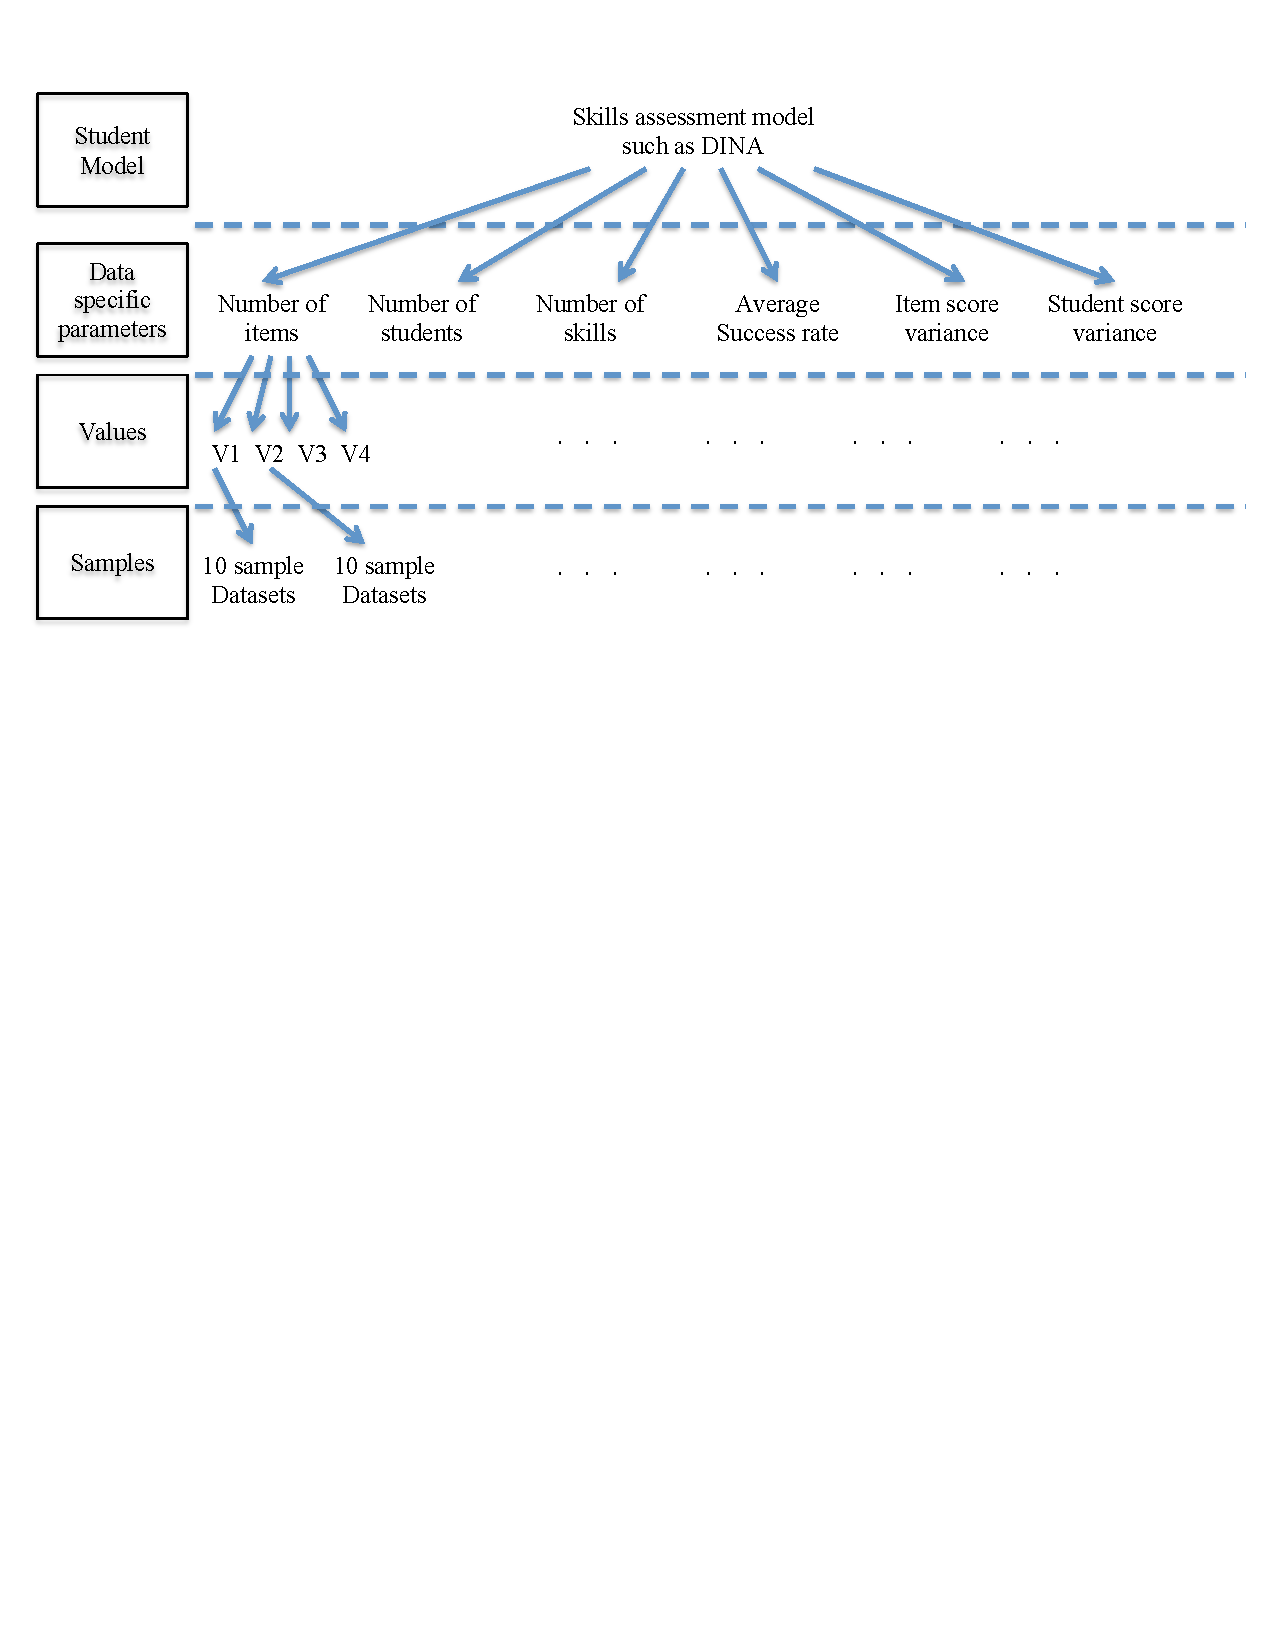
\includegraphics[trim=1cm 17cm 1cm 1cm,scale=0.55]{images/Data-Gen-Break-Down.pdf}
	\onslide<2> 
	\begin{itemize}
	\item Evaluating the ability of the Signature approach to identify the ground truth model \textbf{over datasets with different data specific parameters}
	\item Comparing the results with the best performer approach.
\end{itemize}
	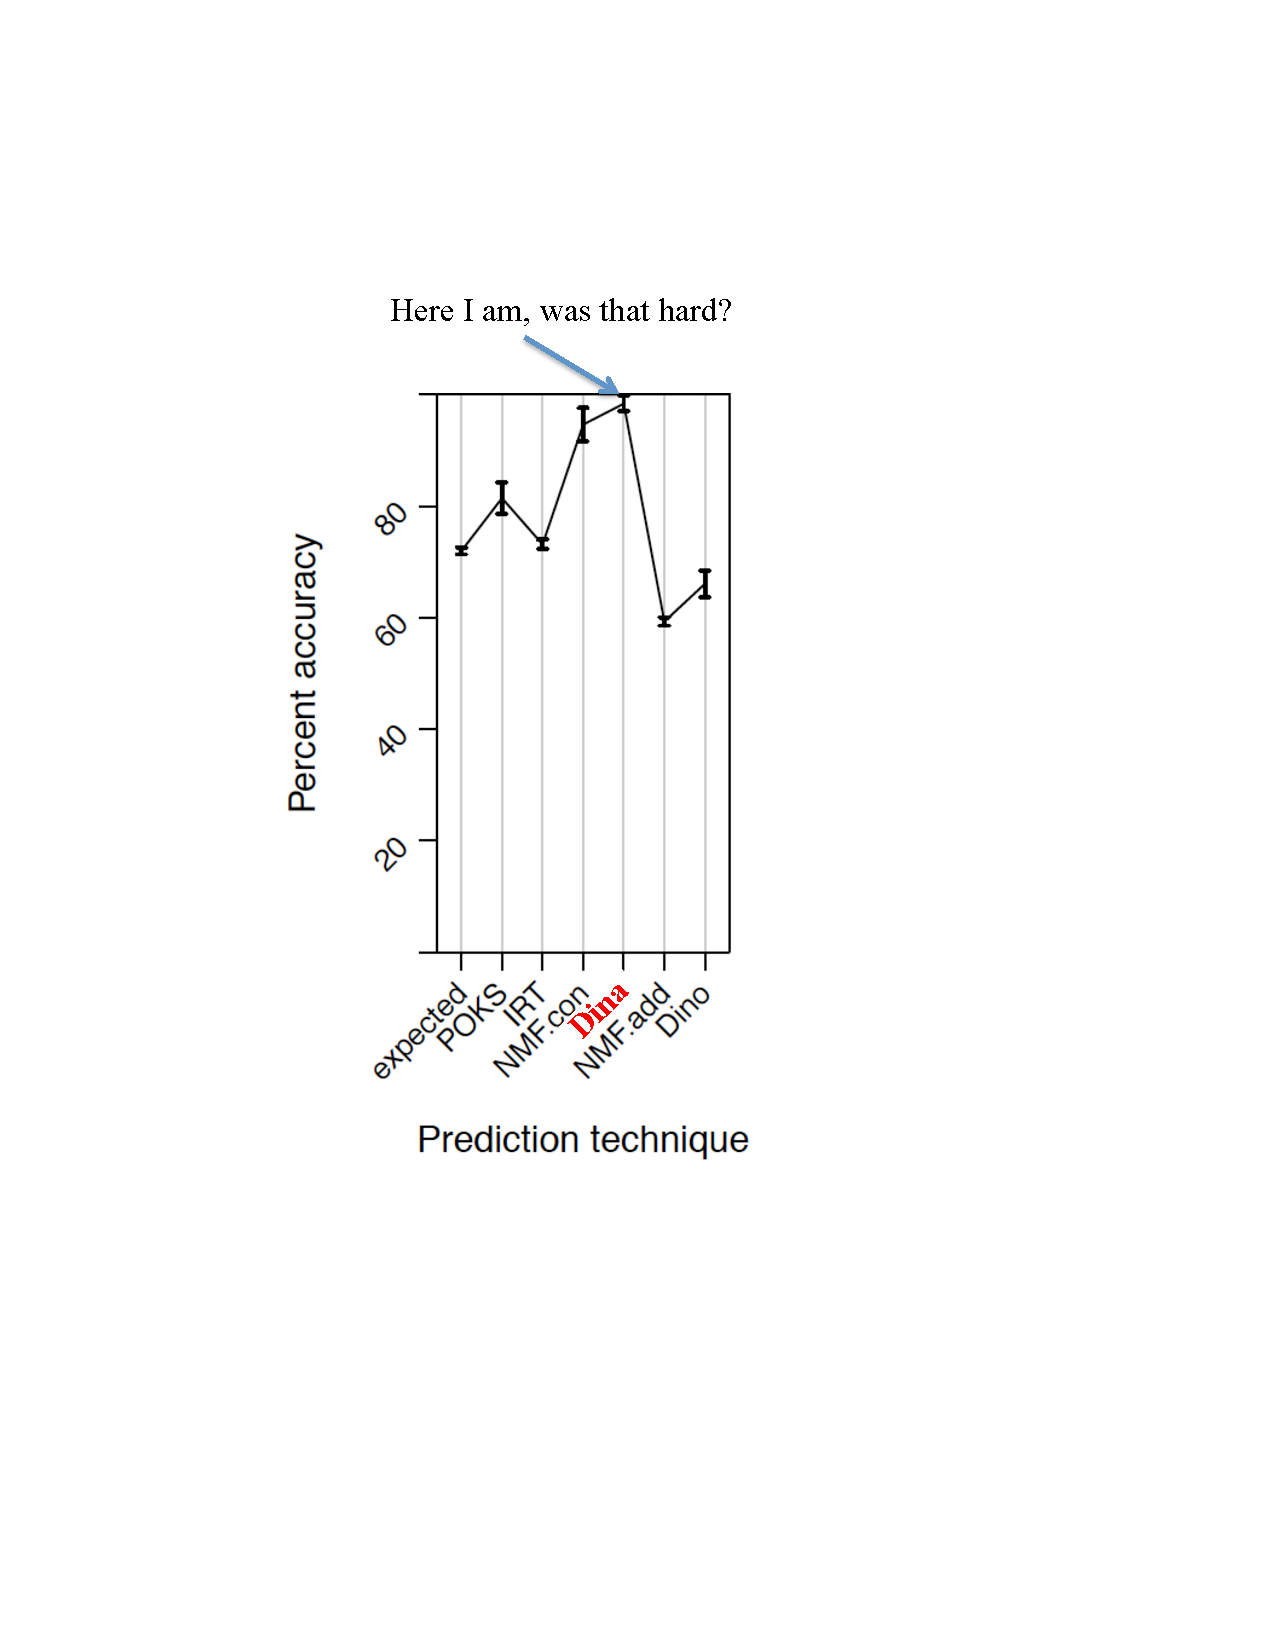
\includegraphics[trim=3cm 10cm 5cm 5cm,scale=0.36]{images/BestPerformer.pdf}
\onslide<3>
\begin{itemize}
	\item Evaluating the ability of the Signature approach to identify the ground truth model \textbf{over datasets with different data specific parameters}
	\item Comparing the results with the best performer approach.
	\item Reporting the accuracy of these classification in terms of precision, recall, F1 measure
\end{itemize}
\begin{columns}
\begin{column}{.4\textwidth}
\vspace{-0.5cm}
\begin{center}
\resizebox{\columnwidth}{!}{\begin{tabular}{c|c|c|c|}
\multicolumn{2}{c}{}&\multicolumn{2}{c}{Prediction outcome}\tabularnewline
\cline{3-4}
\multicolumn{2}{c|}{}& \multicolumn{1}{c|}{Positive} & \multicolumn{1}{c|}{Negative} \tabularnewline
\cline{2-4}
Actual&  \multicolumn{1}{c|}{Positive }&TP&FN\tabularnewline
\cline{2-4}
value& \multicolumn{1}{c|}{Negative} &FP&TN\tabularnewline
\cline{2-4}
\end{tabular}}

\[Precision = \frac{TP}{TP+FP}\]
\[Recall = \frac{TP}{TP+FN}\]

\end{center}
\end{column}
\begin{column}{.6\textwidth}
\vspace{-1cm}
\begin{center}
\[Accuracy = \frac{TP+TN}{TP+TN+FP+FN}\]
\[F_\beta = (1+\beta^2).\frac{Precision.Recall}{\beta^2.Precision+Recall}\]
\end{center}
\end{column}
\end{columns}
\end{overprint}


\end{frame}

\begin{frame}\frametitle{Results of signature vs. best performer classification}
\resizebox{\columnwidth}{!}{\begin{tabular}{c|c|c|c|c|c!{\VRule[2pt]}c|c|c|c|}
\multicolumn{2}{c}{}&\multicolumn{8}{c}{Performance}\tabularnewline
\cline{3-10}
\multicolumn{2}{c|}{}&\multicolumn{4}{c|}{Best Performer}&\multicolumn{4}{c|}{Nearest Neighbor}\tabularnewline
\cline{3-10}
\multicolumn{2}{c|}{}&\scriptsize Precision&\scriptsize Recall&\multicolumn{1}{c|}{\scriptsize F-Measure}&\scriptsize Accuracy&\scriptsize Precision&\scriptsize Recall&\scriptsize F-Measure&\scriptsize Accuracy\tabularnewline
\cline{2-10}
&POKS&0.564&0.992&0.719&0.871&0.793&0.908&\cellcolor{gray!25}0.847&\cellcolor{gray!25}0.945\tabularnewline
\cline{2-10}
&IRT&0.982&0.458&0.625&0.908&0.846&0.867&\cellcolor{gray!25}0.856&\cellcolor{gray!25}0.951\tabularnewline
\cline{2-10}
&NMF Conj.&0.943&0.342&0.502&0.887&0.711&0.750&\cellcolor{gray!25}0.730&\cellcolor{gray!25}0.907\tabularnewline
\cline{2-10}
&DINA&0.617&0.921&0.739&0.891&0.777&0.696&\cellcolor{gray!25}0.734&\cellcolor{gray!25}0.916\tabularnewline
\cline{2-10}
&NMF Add.&0.938&0.875&0.905&0.969&0.946&0.879&\cellcolor{gray!25}0.911&\cellcolor{gray!25}0.971\tabularnewline
\cline{2-10}
\multicolumn{1}{c|}{\multirow{-7}{*}{\begin{sideways}Models\end{sideways}}}&DINO&1&0.929&0.963&0.988&0.996&0.946&\cellcolor{gray!25}0.970&\cellcolor{gray!25}0.990\tabularnewline
\cline{1-10}
\multicolumn{2}{|c|}{Total accuracy}&\multicolumn{4}{c|}{0.75\%}&\multicolumn{4}{c|}{\cellcolor{gray!25}0.84\%}\tabularnewline
\cline{1-10}
\end{tabular}}
\begin{itemize}
\item The F-measure increases when the signature approach is used for classification.\pause
\item In terms of individual scores per method, the accuracy increases when signature approach is used.\pause
\item The total accuracy considers true positive numbers over number of datasets regardless of individual models
\end{itemize}
\end{frame}

\section{Conclusion}
\begin{frame}\frametitle{Research questions}
\begin{enumerate}
\item \checkmark What is the \textit{performance vector} of student skills assessment models over real and over synthetic data created using the same models?
\begin{itemize}
\item Experiment 1: Predictive performance of models over real and synthetic data sets
\end{itemize}
\item \checkmark Is the \textit{performance vector} unique to each synthetic data type (data from the same ground truth model)?
\begin{itemize}
\item Experiment 2: Sensitivity of the Model performance over different data generation parameters
\end{itemize}
\item \checkmark Can the \textit{performance vector} be used to define a method to reliably identify the ground truth behind the synthetic data?
\begin{itemize}
\item Experiment 3: Model selection based on performance vector classification
\end{itemize}
\item \checkmark How does the method compare with the standard practice of using the model with the best performance?
\begin{itemize}
\item Experiment 4: Signature vs. best performer classification
\end{itemize}
\end{enumerate}

\end{frame}

\subsection{Conclusion and discussion}
\begin{frame}\frametitle{Conclusion}
\begin{itemize}
\item Model fit of a data set is defined as the similarity between \textit{prototype} and \textit{target} performance vector \pause
\item The generative model does not always correspond to the best performer and our approach provides a more reliable means \pause
%This means of determining a data set’s ground truth is made possible because the synthetic data sets have very distinct performance patterns, showing sharp differences across models. and uniqueness characteristics
\item Datasets that share a common source have correlated performance vectors. \pause % Fraction data
\item It does not seem to substantially extend to data that shares the same domain
\end{itemize}
\end{frame}

\begin{frame}\frametitle{Conclusion}
\begin{itemize}
\item For real data sets, the performances are not better than the expected performance \pause %the conclusion behind that can be either the ground truth is not among the candidate models, or the best performer is not necessarily the ground truth.
\item For synthetic  data, datasets with different ground truths that share some concepts, show a high correlation. \pause
\item \textit{performance vector} changes for some data specific parameters but it still shows a high correlation with datasets with the same ground truth. \pause
\item Best performer may not be the model that is most representative of the ground truth.
\end{itemize}
\end{frame}

\subsection{Future works}
\begin{frame}\frametitle{Future works}
\begin{itemize}
\item Further studies with real and simulated data \pause
\item generalize to dynamic data and skills assessment models \pause
\item Candidate models and their complexity \pause
\item Application in other fields of study  
\end{itemize}
\end{frame}
\subsection{Questions}
\begin{frame}\frametitle{Thank you}
\begin{figure}

\includegraphics[scale =0.55] {images/Question} 
\end{figure}
\end{frame}
\end{document}

%Pardos Work compared with our work : make link between performance space and parameter space.  We look for close points of synthetic data, they look for similar likelihood surfaces in the space of parameters
